%% LyX 2.2.3 created this file.  For more info, see http://www.lyx.org/.
%% Do not edit unless you really know what you are doing.
\documentclass[12pt,oneside,american,english,italian]{book}
\renewcommand{\familydefault}{\rmdefault}
\usepackage[T1]{fontenc}
\usepackage[latin9]{luainputenc}
\usepackage{geometry}
\geometry{verbose,tmargin=2.5cm,bmargin=2cm,lmargin=2cm,rmargin=2cm}
\setcounter{secnumdepth}{3}
\setcounter{tocdepth}{3}
\usepackage{color}
\usepackage{array}
\usepackage{verbatim}
\usepackage{longtable}
\usepackage{float}
\usepackage{amssymb}
\usepackage{graphicx}

\makeatletter

%%%%%%%%%%%%%%%%%%%%%%%%%%%%%% LyX specific LaTeX commands.
%% Because html converters don't know tabularnewline
\providecommand{\tabularnewline}{\\}

%%%%%%%%%%%%%%%%%%%%%%%%%%%%%% User specified LaTeX commands.
% LOGO
\usepackage{eso-pic,graphicx}
\makeatletter
\newcommand\BackgroundPicture[2]{
\setlength{\unitlength}{1pt}
\put(0,\strip@pt\paperheight){
\parbox[t][\paperheight]{\paperwidth}{
\vfill
\centering\includegraphics[angle=#2]{#1}
\vfill
}
}
}
\makeatother
%Per i marigini
\sloppy

\usepackage{listings,xcolor,courier,bookmark}
\usepackage{listingsutf8}
\definecolor{darkblue}{named}{blue}
\definecolor{darkred}{named}{red}
\definecolor{grau}{named}{gray}
\let\Righttorque\relax
\lstset{
captionpos=b,
commentstyle=\color[rgb]{0.133,0.545,0.133},
keywordstyle=\color{darkblue},
stringstyle=\color{darkred},
extendedchars=true,
basicstyle=\small\ttfamily,
showstringspaces=false,
tabsize=2,
numbers=left,
numberstyle=\tiny,
breakautoindent  = true,
breakindent      = 2em,
breaklines       = true,
postbreak        = ,
prebreak         = \raisebox{-.8ex}[0ex][0ex]{\Righttorque},
showspaces=false, 
showtabs=false, 
showstringspaces=false,
language=VHDL,
frame=single,
morecomment=[s]{--}
}


\renewcommand*{\lstlistingname}{Codice Componente}

\usepackage{fancyhdr}
\pagestyle{fancy}

\fancyhead{} % cancella tutti i campi
\fancyfoot{} % cancella tutti i campi

\fancyhead[RO,LE]{\bfseries \leftmark}
\fancyfoot[LE,RO]{\thepage}
\fancyfoot[LO,CE]{Elaborato di ASE: Architettura dei Sistemi di Elaborazione}
\renewcommand{\headrulewidth}{0.4pt}
\renewcommand{\footrulewidth}{0.4pt}
\cfoot{}
\usepackage{tikz}
\usetikzlibrary{matrix,calc}

%isolated term
%#1 - Optional. Space between node and grouping line. Default=0
%#2 - node
%#3 - filling color
\newcommand{\implicantsol}[3][0]{
    \draw[rounded corners=3pt, fill=#3, opacity=0.3] ($(#2.north west)+(135:#1)$) rectangle ($(#2.south east)+(-45:#1)$);
    }


%internal group
%#1 - Optional. Space between node and grouping line. Default=0
%#2 - top left node
%#3 - bottom right node
%#4 - filling color
\newcommand{\implicant}[4][0]{
    \draw[rounded corners=3pt, fill=#4, opacity=0.3] ($(#2.north west)+(135:#1)$) rectangle ($(#3.south east)+(-45:#1)$);
    }

%group lateral borders
%#1 - Optional. Space between node and grouping line. Default=0
%#2 - top left node
%#3 - bottom right node
%#4 - filling color
\newcommand{\implicantcostats}[4][0]{
    \draw[rounded corners=3pt, fill=#4, opacity=0.3] ($(rf.east |- #2.north)+(90:#1)$)-| ($(#2.east)+(0:#1)$) |- ($(rf.east |- #3.south)+(-90:#1)$);
    \draw[rounded corners=3pt, fill=#4, opacity=0.3] ($(cf.west |- #2.north)+(90:#1)$) -| ($(#3.west)+(180:#1)$) |- ($(cf.west |- #3.south)+(-90:#1)$);
}

%group top-bottom borders
%#1 - Optional. Space between node and grouping line. Default=0
%#2 - top left node
%#3 - bottom right node
%#4 - filling color
\newcommand{\implicantdaltbaix}[4][0]{
    \draw[rounded corners=3pt, fill=#4, opacity=0.3] ($(cf.south -| #2.west)+(180:#1)$) |- ($(#2.south)+(-90:#1)$) -| ($(cf.south -| #3.east)+(0:#1)$);
    \draw[rounded corners=3pt, fill=#4, opacity=0.3] ($(rf.north -| #2.west)+(180:#1)$) |- ($(#3.north)+(90:#1)$) -| ($(rf.north -| #3.east)+(0:#1)$);
}

%group corners
%#1 - Optional. Space between node and grouping line. Default=0
%#2 - filling color
\newcommand{\implicantcantons}[2][0]{
    \draw[rounded corners=3pt, opacity=.3] ($(rf.east |- 0.south)+(-90:#1)$) -| ($(0.east |- cf.south)+(0:#1)$);
    \draw[rounded corners=3pt, opacity=.3] ($(rf.east |- 8.north)+(90:#1)$) -| ($(8.east |- rf.north)+(0:#1)$);
    \draw[rounded corners=3pt, opacity=.3] ($(cf.west |- 2.south)+(-90:#1)$) -| ($(2.west |- cf.south)+(180:#1)$);
    \draw[rounded corners=3pt, opacity=.3] ($(cf.west |- 10.north)+(90:#1)$) -| ($(10.west |- rf.north)+(180:#1)$);
    \fill[rounded corners=3pt, fill=#2, opacity=.3] ($(rf.east |- 0.south)+(-90:#1)$) -|  ($(0.east |- cf.south)+(0:#1)$) [sharp corners] ($(rf.east |- 0.south)+(-90:#1)$) |-  ($(0.east |- cf.south)+(0:#1)$) ;
    \fill[rounded corners=3pt, fill=#2, opacity=.3] ($(rf.east |- 8.north)+(90:#1)$) -| ($(8.east |- rf.north)+(0:#1)$) [sharp corners] ($(rf.east |- 8.north)+(90:#1)$) |- ($(8.east |- rf.north)+(0:#1)$) ;
    \fill[rounded corners=3pt, fill=#2, opacity=.3] ($(cf.west |- 2.south)+(-90:#1)$) -| ($(2.west |- cf.south)+(180:#1)$) [sharp corners]($(cf.west |- 2.south)+(-90:#1)$) |- ($(2.west |- cf.south)+(180:#1)$) ;
    \fill[rounded corners=3pt, fill=#2, opacity=.3] ($(cf.west |- 10.north)+(90:#1)$) -| ($(10.west |- rf.north)+(180:#1)$) [sharp corners] ($(cf.west |- 10.north)+(90:#1)$) |- ($(10.west |- rf.north)+(180:#1)$) ;
}

%Empty Karnaugh map 4x4
\newenvironment{Karnaugh}%
{
\begin{tikzpicture}[baseline=(current bounding box.north),scale=0.8]
\draw (0,0) grid (4,4);
\draw (0,4) -- node [pos=0.7,above right,anchor=south west] {cd} node [pos=0.7,below left,anchor=north east] {ab} ++(135:1);
%
\matrix (mapa) [matrix of nodes,
        column sep={0.8cm,between origins},
        row sep={0.8cm,between origins},
        every node/.style={minimum size=0.3mm},
        anchor=8.center,
        ampersand replacement=\&] at (0.5,0.5)
{
                       \& |(c00)| 00         \& |(c01)| 01         \& |(c11)| 11         \& |(c10)| 10         \& |(cf)| \phantom{00} \\
|(r00)| 00             \& |(0)|  \phantom{0} \& |(1)|  \phantom{0} \& |(3)|  \phantom{0} \& |(2)|  \phantom{0} \&                     \\
|(r01)| 01             \& |(4)|  \phantom{0} \& |(5)|  \phantom{0} \& |(7)|  \phantom{0} \& |(6)|  \phantom{0} \&                     \\
|(r11)| 11             \& |(12)| \phantom{0} \& |(13)| \phantom{0} \& |(15)| \phantom{0} \& |(14)| \phantom{0} \&                     \\
|(r10)| 10             \& |(8)|  \phantom{0} \& |(9)|  \phantom{0} \& |(11)| \phantom{0} \& |(10)| \phantom{0} \&                     \\
|(rf) | \phantom{00}   \&                    \&                    \&                    \&                    \&                     \\
};
}%
{
\end{tikzpicture}
}

%Empty Karnaugh map 2x4
\newenvironment{Karnaughvuit}%
{
\begin{tikzpicture}[baseline=(current bounding box.north),scale=0.8]
\draw (0,0) grid (4,2);
\draw (0,2) -- node [pos=0.7,above right,anchor=south west] {bc} node [pos=0.7,below left,anchor=north east] {a} ++(135:1);
%
\matrix (mapa) [matrix of nodes,
        column sep={0.8cm,between origins},
        row sep={0.8cm,between origins},
        every node/.style={minimum size=0.3mm},
        anchor=4.center,
        ampersand replacement=\&] at (0.5,0.5)
{
                      \& |(c00)| 00         \& |(c01)| 01         \& |(c11)| 11         \& |(c10)| 10         \& |(cf)| \phantom{00} \\
|(r00)| 0             \& |(0)|  \phantom{0} \& |(1)|  \phantom{0} \& |(3)|  \phantom{0} \& |(2)|  \phantom{0} \&                     \\
|(r01)| 1             \& |(4)|  \phantom{0} \& |(5)|  \phantom{0} \& |(7)|  \phantom{0} \& |(6)|  \phantom{0} \&                     \\
|(rf) | \phantom{00}  \&                    \&                    \&                    \&                    \&                     \\
};
}%
{
\end{tikzpicture}
}

%Empty Karnaugh map 2x2
\newenvironment{Karnaughquatre}%
{
\begin{tikzpicture}[baseline=(current bounding box.north),scale=0.8]
\draw (0,0) grid (2,2);
\draw (0,2) -- node [pos=0.7,above right,anchor=south west] {b} node [pos=0.7,below left,anchor=north east] {a} ++(135:1);
%
\matrix (mapa) [matrix of nodes,
        column sep={0.8cm,between origins},
        row sep={0.8cm,between origins},
        every node/.style={minimum size=0.3mm},
        anchor=2.center,
        ampersand replacement=\&] at (0.5,0.5)
{
          \& |(c00)| 0          \& |(c01)| 1  \\
|(r00)| 0 \& |(0)|  \phantom{0} \& |(1)|  \phantom{0} \\
|(r01)| 1 \& |(2)|  \phantom{0} \& |(3)|  \phantom{0} \\
};
}%
{
\end{tikzpicture}
}

%Defines 8 or 16 values (0,1,X)
\newcommand{\contingut}[1]{%
\foreach \x [count=\xi from 0]  in {#1}
     \path (\xi) node {\x};
}

%Places 1 in listed positions
\newcommand{\minterms}[1]{%
    \foreach \x in {#1}
        \path (\x) node {1};
}

%Places 0 in listed positions
\newcommand{\maxterms}[1]{%
    \foreach \x in {#1}
        \path (\x) node {0};
}

%Places X in listed positions
\newcommand{\indeterminats}[1]{%
    \foreach \x in {#1}
        \path (\x) node {X};
}
\hypersetup{hidelinks}
\usepackage[italian]{varioref}
\usepackage{caption}
\colorlet{BLACK}{black}
\captionsetup{tableposition=top,figureposition=bottom,font=small,format=hang,labelfont={sf,bf}}
\usepackage{hyperref}

\makeatother

\usepackage{babel}
\begin{document}
\begin{frontmatter}
\pagenumbering{Roman}

\title{Tesina di Architettura dei Sistemi di Elaborazione \\Gruppo 4} 

\author{Milo Saverio - Mat. M63/XXXX
\and Pommella Michele - Mat. M63/XXXX
\and Trimaldi Davide - Mat. M63/XXXX
}

\maketitle

\setcounter{page}{1}

\pagebreak{}

\tableofcontents{}

\pagebreak{}

\selectlanguage{american}%
\end{frontmatter}

\begin{mainmatter}

\selectlanguage{italian}%

\chapter{\textcolor{black}{Minimizzazione} reti combinatorie }

\selectlanguage{american}%

\AddToShipoutPicture{\BackgroundPicture{logo.png}{0}}

\selectlanguage{italian}%

\section{Traccia}

Realizzare un dispositivo VHDL che implementa il protocollo UART (a
partire da quello diffuso dalla Digilent). Collegare internamente,
oppure tramite inter- faccia fisica esterna alla board stessa, ad
un\textquoteright altra board oppure ad un PC previo utilizzo di un
physical RS232, due interfacce per trasmette e ricevere ottetti. Svolgere
l\textquoteright esercizio riutilizzando il VHDL messo a disposizione
da Digilent (e disponbile nel materiale del corso) commentando eventuali
ristrutturazioni del codice. (Opzionale) Sviluppare un\textquoteright architettura
per l\textquoteright implementazione del protocollo UART secondo il
paradigma PO/PC ex-novo, evidenziando le similarit`a/dissimilarit`a
con il progetto Digilent.\selectlanguage{italian}%



\selectlanguage{italian}%

\section{Soluzione}


\subsection{Schematici}

Il seguente circuito implementa l' algortimo RSA per la firma di un
messaggio, applica una funzione di hash sul messaggio e verifica che
il messaggio ricevuto sia coretto.

L' intera procedura � divisa nelle seguenti fasi: 
\begin{itemize}
\item vengono scelti i valori caratteristici per inviare il dato (p pari
a 3, q 11, e 7 e d 3) ed il messaggio da inviare;
\item si applica la funzione di hashing sul messaggio, utilizzando il metodo
della moltiplicazione;
\item viene applicata la firma sul messaggio originale utilizzando la chiave
privata, il trasmettitore invia i due dati appena calcolati (anche
se non � presente un vero e proprio invio essendo trasmettitore e
ricevitore implementati sulla stessa board);
\item Il ricevitore applica la chiave pubblica sul messaggio firmato, ne
effettua l' hashing e verifica se la sua versione del messaggio a
cui � stato applicato l' hashing � identico a quello che � stato ricevuto.
\end{itemize}
Cos� facendo garantiamo sia la segretezza( infatti non mandiamo il
messaggio in chiaro), sia l' autenticazione( chi riceve il messaggio
pu� verificare effettuando l' hashing con parametri convenuti non
� stato modificato),

Di seguito vengono descritte le varie componenti che vengono utilizzate
per effettuare l' hashing e firmare il messaggio.

\subsubsection{Funzione hash}

\begin{figure}[H]
	\centering
	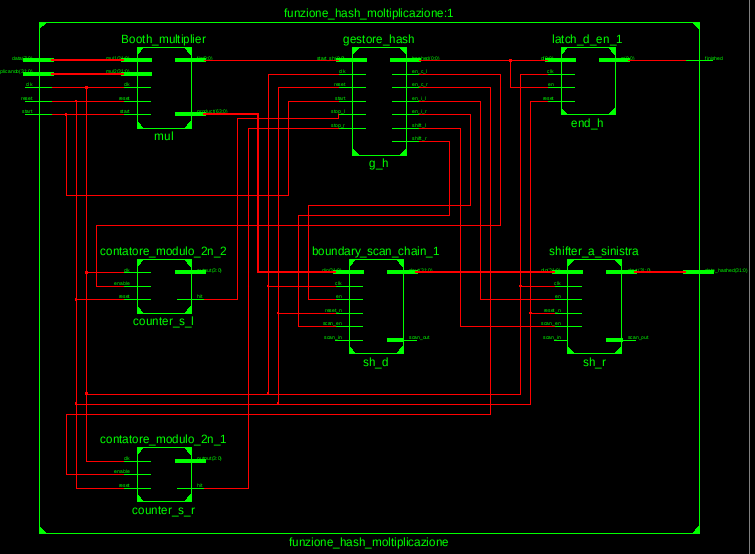
\includegraphics[scale=0.6]{esercizio17/images/hash.png}
	\caption{hasher}
	\label{fig:Mod_exp}
\end{figure}Il circuito � stato realizzato in due differenti modi: 
\begin{itemize}
\item nel primo caso si utilizza una macchina a stati finiti descritta da
cinque stati: 
\begin{itemize}
\item idle, stato di riposo dell' automa; 
\item init in cui si attende che il moltiplicatore termini il suo compito; 
\item shifting\_r in cui il valore della moltiplicazione viene shiftato
a destra; 
\item shifting\_l il valore viene shiftato a sinistra; ended per comunicare
la fine dell' operazione di hash;
\end{itemize}
\item nel secondo si � utilizzato lo stesso procedimento ma il tutto viene
implementato in un process.
\end{itemize}
Viene utilizzata la seconda soluzione perch� occupa meno spazio, dato
che le operazioni di shifting consistono semplicemente, nel caso dello
shifting a destra prendere i sedici bit pi� significativi dal risultato
della moltiplicazione, quando si shifta a sinistra basta accodare
sedici zeri per avere lo stesso risultato della prima soluzione.

Il circito viene cos� descritto poich� tale forma di hashing prevedere
di moltiplicare il dato per un valore A il quale � un numero compreso
tra 0 ed 1, di cui il denominatore � un multiplo di due, per tale
ragione di � scelto di moltiplicare per un valore W ed infine di shiftare
a destra un numero di volte pari al valore dell' esponente, tale numero
� la parte decimale del valore del dato per W (perch� quando shiftiamo
inseriamo degli zero fittizzi), dopodich� si effettua uno shifting
a sinistra di un numero pari di volte affinch� la nostra parte deciamale
rientri nella parte del registro da inviare.

\subsubsection{Esponenziatore}

Per effettuare l' elevazione a potenza con il modulo, ci siamo riferiti
a questo algoritmo :

\begin{figure}[H]
	\centering
	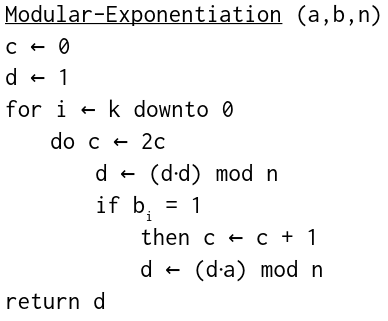
\includegraphics[scale=0.8]{esercizio17/images/mod_exp.png}
	\caption{Algoritmo per modular exponentiational di un messaggio}
	\label{fig:Mod_exp}
\end{figure}

L ' algoritmo cicla sul numero di bit dell ' esponente, moltiplica
il valore d prima per se stesso e ne fa il modulo, questo stesso valore
di d per la base quando il valore dell' esponente in forma binaria
assume valore uno e ne effettua il modulo, (il parametro c non occorre
per il calcolo del valore finale, occorre solo a capire in realt�
alla fine se il numero � stato elevato per il corretto esponente). 

\begin{figure}[H]
	\centering
	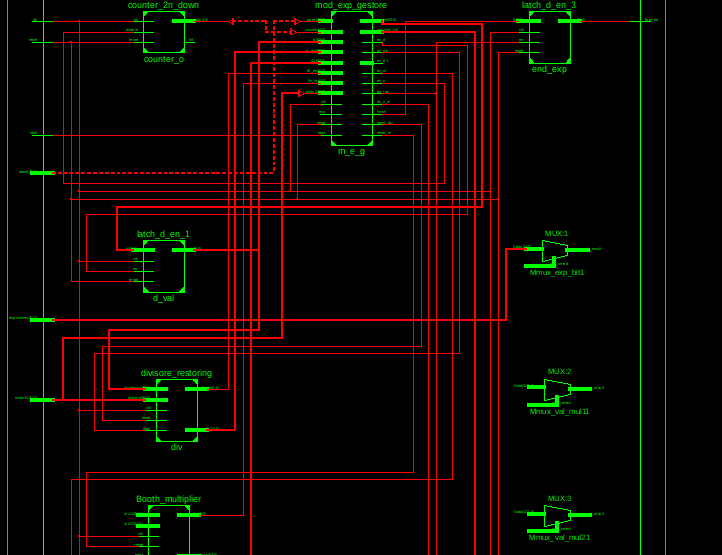
\includegraphics[scale=0.6]{esercizio17/images/exp.png}
	\caption{Hardware Exponentiational}
\end{figure}

Utiliziamo questo algoritmo perch� ci permette di riutilizzare componenti
gi� sviluppati negli esercizi precedenti, difatti osservando lo schematico,
vi � presente un moltiplicatore di Booth e il divisore restoring per
le varie operazioni prodotto e modulo, un contatore down per indicare
quale dei bit dell' esponente dobbiamo analizzare e dei selettori
descritti con il costrutto with select per selezionare quali valori
devono essere moltiplicati. La macchina a stati finiti non fa altro
che eseguire i vari passi dell' algoritmo, per� per problemi relativi
al timing � stata realizzata alla fine con un singolo process, difatti
una prima realizzazione con due process determinava che alcuni registri
contenti i dati dell' operazione assumessero un valore indefinito
(veniva sintetizzata un macchina che doveva avere una frequenza di
clock minore da quella generabile dalla scheda). 

Per problemi di spazio, si � ricorsi a componenti per la moltiplicazione
e divisione seriali, oltre ad riutilizzarli all' interno dello stesso
progetto difatti il moltiplicatore di Booth � stato utilizzato per:
calcolare il prodotto di pq ed l' esponenziazione.

\subsection{Codice}

\href{run:progetti/RSA/RSA.xise}{RSA ISE}

\selectlanguage{italian}%



\selectlanguage{italian}%

\section{Simulazione}

\begin{figure}[H]
	\centering
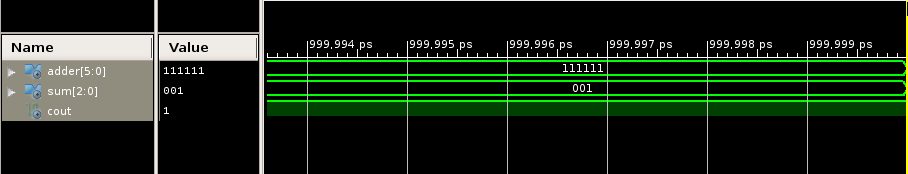
\includegraphics[scale=0.55]{esercizio10/images/carry_save_adder_testbench.png}
	\caption{Carry Save Adder}
\end{figure}\selectlanguage{italian}%



\selectlanguage{italian}%

\section{Sintesi su board FPGA}

Valgono le stesse considerazioni fatte per il Ripple Carry Adder \ref{Sintesi ripple carry},
con la differenza che ci sono sette registri da poter caricare.\selectlanguage{italian}%

\selectlanguage{italian}%



\chapter{Reti combinatorie con l'ausilio di SIS e Mapping Tecnologico}

\selectlanguage{american}%

\AddToShipoutPicture{\BackgroundPicture{logo.png}{0}}

\selectlanguage{italian}%

\section{Traccia}

Realizzare un dispositivo VHDL che implementa il protocollo UART (a
partire da quello diffuso dalla Digilent). Collegare internamente,
oppure tramite inter- faccia fisica esterna alla board stessa, ad
un\textquoteright altra board oppure ad un PC previo utilizzo di un
physical RS232, due interfacce per trasmette e ricevere ottetti. Svolgere
l\textquoteright esercizio riutilizzando il VHDL messo a disposizione
da Digilent (e disponbile nel materiale del corso) commentando eventuali
ristrutturazioni del codice. (Opzionale) Sviluppare un\textquoteright architettura
per l\textquoteright implementazione del protocollo UART secondo il
paradigma PO/PC ex-novo, evidenziando le similarit`a/dissimilarit`a
con il progetto Digilent.\selectlanguage{italian}%



\selectlanguage{italian}%

\section{Soluzione}


\subsection{Schematici}

Il seguente circuito implementa l' algortimo RSA per la firma di un
messaggio, applica una funzione di hash sul messaggio e verifica che
il messaggio ricevuto sia coretto.

L' intera procedura � divisa nelle seguenti fasi: 
\begin{itemize}
\item vengono scelti i valori caratteristici per inviare il dato (p pari
a 3, q 11, e 7 e d 3) ed il messaggio da inviare;
\item si applica la funzione di hashing sul messaggio, utilizzando il metodo
della moltiplicazione;
\item viene applicata la firma sul messaggio originale utilizzando la chiave
privata, il trasmettitore invia i due dati appena calcolati (anche
se non � presente un vero e proprio invio essendo trasmettitore e
ricevitore implementati sulla stessa board);
\item Il ricevitore applica la chiave pubblica sul messaggio firmato, ne
effettua l' hashing e verifica se la sua versione del messaggio a
cui � stato applicato l' hashing � identico a quello che � stato ricevuto.
\end{itemize}
Cos� facendo garantiamo sia la segretezza( infatti non mandiamo il
messaggio in chiaro), sia l' autenticazione( chi riceve il messaggio
pu� verificare effettuando l' hashing con parametri convenuti non
� stato modificato),

Di seguito vengono descritte le varie componenti che vengono utilizzate
per effettuare l' hashing e firmare il messaggio.

\subsubsection{Funzione hash}

\begin{figure}[H]
	\centering
	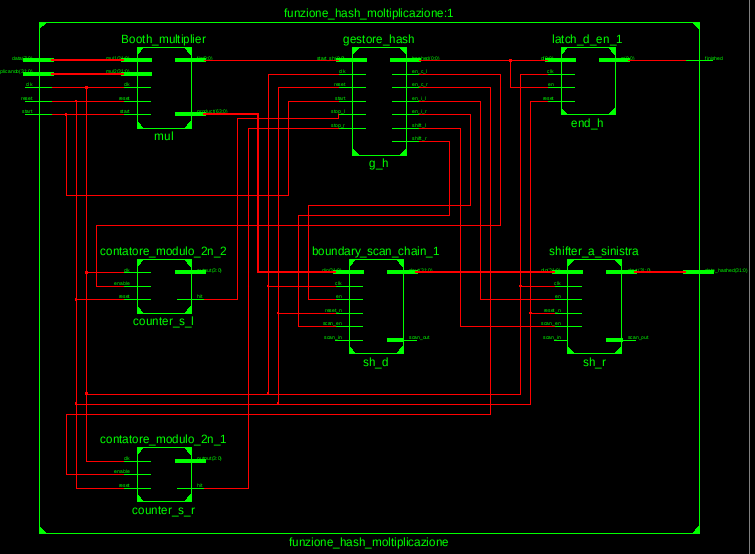
\includegraphics[scale=0.6]{esercizio17/images/hash.png}
	\caption{hasher}
	\label{fig:Mod_exp}
\end{figure}Il circuito � stato realizzato in due differenti modi: 
\begin{itemize}
\item nel primo caso si utilizza una macchina a stati finiti descritta da
cinque stati: 
\begin{itemize}
\item idle, stato di riposo dell' automa; 
\item init in cui si attende che il moltiplicatore termini il suo compito; 
\item shifting\_r in cui il valore della moltiplicazione viene shiftato
a destra; 
\item shifting\_l il valore viene shiftato a sinistra; ended per comunicare
la fine dell' operazione di hash;
\end{itemize}
\item nel secondo si � utilizzato lo stesso procedimento ma il tutto viene
implementato in un process.
\end{itemize}
Viene utilizzata la seconda soluzione perch� occupa meno spazio, dato
che le operazioni di shifting consistono semplicemente, nel caso dello
shifting a destra prendere i sedici bit pi� significativi dal risultato
della moltiplicazione, quando si shifta a sinistra basta accodare
sedici zeri per avere lo stesso risultato della prima soluzione.

Il circito viene cos� descritto poich� tale forma di hashing prevedere
di moltiplicare il dato per un valore A il quale � un numero compreso
tra 0 ed 1, di cui il denominatore � un multiplo di due, per tale
ragione di � scelto di moltiplicare per un valore W ed infine di shiftare
a destra un numero di volte pari al valore dell' esponente, tale numero
� la parte decimale del valore del dato per W (perch� quando shiftiamo
inseriamo degli zero fittizzi), dopodich� si effettua uno shifting
a sinistra di un numero pari di volte affinch� la nostra parte deciamale
rientri nella parte del registro da inviare.

\subsubsection{Esponenziatore}

Per effettuare l' elevazione a potenza con il modulo, ci siamo riferiti
a questo algoritmo :

\begin{figure}[H]
	\centering
	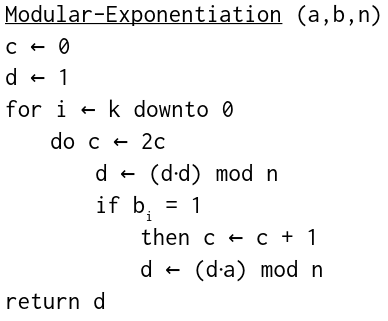
\includegraphics[scale=0.8]{esercizio17/images/mod_exp.png}
	\caption{Algoritmo per modular exponentiational di un messaggio}
	\label{fig:Mod_exp}
\end{figure}

L ' algoritmo cicla sul numero di bit dell ' esponente, moltiplica
il valore d prima per se stesso e ne fa il modulo, questo stesso valore
di d per la base quando il valore dell' esponente in forma binaria
assume valore uno e ne effettua il modulo, (il parametro c non occorre
per il calcolo del valore finale, occorre solo a capire in realt�
alla fine se il numero � stato elevato per il corretto esponente). 

\begin{figure}[H]
	\centering
	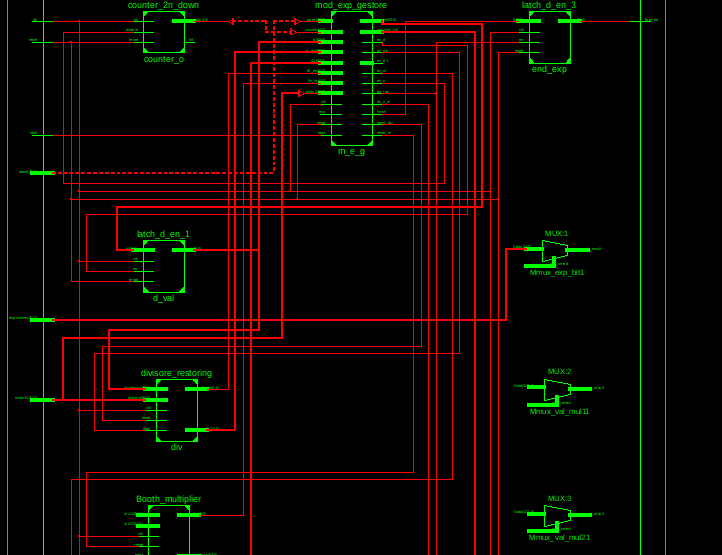
\includegraphics[scale=0.6]{esercizio17/images/exp.png}
	\caption{Hardware Exponentiational}
\end{figure}

Utiliziamo questo algoritmo perch� ci permette di riutilizzare componenti
gi� sviluppati negli esercizi precedenti, difatti osservando lo schematico,
vi � presente un moltiplicatore di Booth e il divisore restoring per
le varie operazioni prodotto e modulo, un contatore down per indicare
quale dei bit dell' esponente dobbiamo analizzare e dei selettori
descritti con il costrutto with select per selezionare quali valori
devono essere moltiplicati. La macchina a stati finiti non fa altro
che eseguire i vari passi dell' algoritmo, per� per problemi relativi
al timing � stata realizzata alla fine con un singolo process, difatti
una prima realizzazione con due process determinava che alcuni registri
contenti i dati dell' operazione assumessero un valore indefinito
(veniva sintetizzata un macchina che doveva avere una frequenza di
clock minore da quella generabile dalla scheda). 

Per problemi di spazio, si � ricorsi a componenti per la moltiplicazione
e divisione seriali, oltre ad riutilizzarli all' interno dello stesso
progetto difatti il moltiplicatore di Booth � stato utilizzato per:
calcolare il prodotto di pq ed l' esponenziazione.

\subsection{Codice}

\href{run:progetti/RSA/RSA.xise}{RSA ISE}

\selectlanguage{italian}%



\selectlanguage{italian}%

\section{Simulazione}

\begin{figure}[H]
	\centering
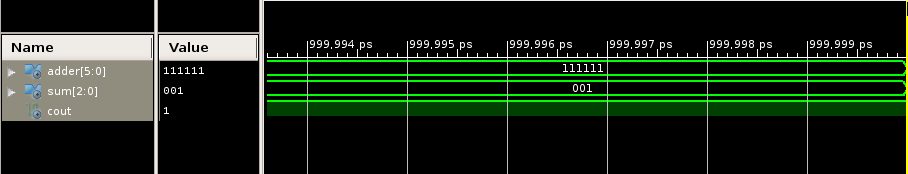
\includegraphics[scale=0.55]{esercizio10/images/carry_save_adder_testbench.png}
	\caption{Carry Save Adder}
\end{figure}\selectlanguage{italian}%



\selectlanguage{italian}%

\section{Sintesi su board FPGA}

Valgono le stesse considerazioni fatte per il Ripple Carry Adder \ref{Sintesi ripple carry},
con la differenza che ci sono sette registri da poter caricare.\selectlanguage{italian}%

\selectlanguage{italian}%



\chapter{Latch/Flip Flop}

\selectlanguage{american}%

\AddToShipoutPicture{\BackgroundPicture{logo.png}{0}}

\selectlanguage{italian}%

\section{Traccia}

Realizzare un dispositivo VHDL che implementa il protocollo UART (a
partire da quello diffuso dalla Digilent). Collegare internamente,
oppure tramite inter- faccia fisica esterna alla board stessa, ad
un\textquoteright altra board oppure ad un PC previo utilizzo di un
physical RS232, due interfacce per trasmette e ricevere ottetti. Svolgere
l\textquoteright esercizio riutilizzando il VHDL messo a disposizione
da Digilent (e disponbile nel materiale del corso) commentando eventuali
ristrutturazioni del codice. (Opzionale) Sviluppare un\textquoteright architettura
per l\textquoteright implementazione del protocollo UART secondo il
paradigma PO/PC ex-novo, evidenziando le similarit`a/dissimilarit`a
con il progetto Digilent.\selectlanguage{italian}%



\selectlanguage{italian}%

\section{Soluzione}


\subsection{Schematici}

Il seguente circuito implementa l' algortimo RSA per la firma di un
messaggio, applica una funzione di hash sul messaggio e verifica che
il messaggio ricevuto sia coretto.

L' intera procedura � divisa nelle seguenti fasi: 
\begin{itemize}
\item vengono scelti i valori caratteristici per inviare il dato (p pari
a 3, q 11, e 7 e d 3) ed il messaggio da inviare;
\item si applica la funzione di hashing sul messaggio, utilizzando il metodo
della moltiplicazione;
\item viene applicata la firma sul messaggio originale utilizzando la chiave
privata, il trasmettitore invia i due dati appena calcolati (anche
se non � presente un vero e proprio invio essendo trasmettitore e
ricevitore implementati sulla stessa board);
\item Il ricevitore applica la chiave pubblica sul messaggio firmato, ne
effettua l' hashing e verifica se la sua versione del messaggio a
cui � stato applicato l' hashing � identico a quello che � stato ricevuto.
\end{itemize}
Cos� facendo garantiamo sia la segretezza( infatti non mandiamo il
messaggio in chiaro), sia l' autenticazione( chi riceve il messaggio
pu� verificare effettuando l' hashing con parametri convenuti non
� stato modificato),

Di seguito vengono descritte le varie componenti che vengono utilizzate
per effettuare l' hashing e firmare il messaggio.

\subsubsection{Funzione hash}

\begin{figure}[H]
	\centering
	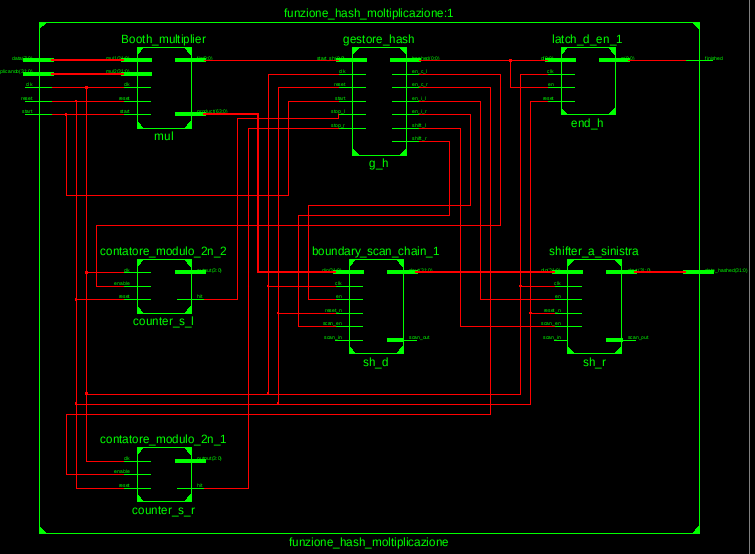
\includegraphics[scale=0.6]{esercizio17/images/hash.png}
	\caption{hasher}
	\label{fig:Mod_exp}
\end{figure}Il circuito � stato realizzato in due differenti modi: 
\begin{itemize}
\item nel primo caso si utilizza una macchina a stati finiti descritta da
cinque stati: 
\begin{itemize}
\item idle, stato di riposo dell' automa; 
\item init in cui si attende che il moltiplicatore termini il suo compito; 
\item shifting\_r in cui il valore della moltiplicazione viene shiftato
a destra; 
\item shifting\_l il valore viene shiftato a sinistra; ended per comunicare
la fine dell' operazione di hash;
\end{itemize}
\item nel secondo si � utilizzato lo stesso procedimento ma il tutto viene
implementato in un process.
\end{itemize}
Viene utilizzata la seconda soluzione perch� occupa meno spazio, dato
che le operazioni di shifting consistono semplicemente, nel caso dello
shifting a destra prendere i sedici bit pi� significativi dal risultato
della moltiplicazione, quando si shifta a sinistra basta accodare
sedici zeri per avere lo stesso risultato della prima soluzione.

Il circito viene cos� descritto poich� tale forma di hashing prevedere
di moltiplicare il dato per un valore A il quale � un numero compreso
tra 0 ed 1, di cui il denominatore � un multiplo di due, per tale
ragione di � scelto di moltiplicare per un valore W ed infine di shiftare
a destra un numero di volte pari al valore dell' esponente, tale numero
� la parte decimale del valore del dato per W (perch� quando shiftiamo
inseriamo degli zero fittizzi), dopodich� si effettua uno shifting
a sinistra di un numero pari di volte affinch� la nostra parte deciamale
rientri nella parte del registro da inviare.

\subsubsection{Esponenziatore}

Per effettuare l' elevazione a potenza con il modulo, ci siamo riferiti
a questo algoritmo :

\begin{figure}[H]
	\centering
	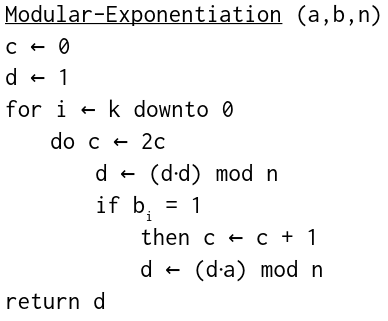
\includegraphics[scale=0.8]{esercizio17/images/mod_exp.png}
	\caption{Algoritmo per modular exponentiational di un messaggio}
	\label{fig:Mod_exp}
\end{figure}

L ' algoritmo cicla sul numero di bit dell ' esponente, moltiplica
il valore d prima per se stesso e ne fa il modulo, questo stesso valore
di d per la base quando il valore dell' esponente in forma binaria
assume valore uno e ne effettua il modulo, (il parametro c non occorre
per il calcolo del valore finale, occorre solo a capire in realt�
alla fine se il numero � stato elevato per il corretto esponente). 

\begin{figure}[H]
	\centering
	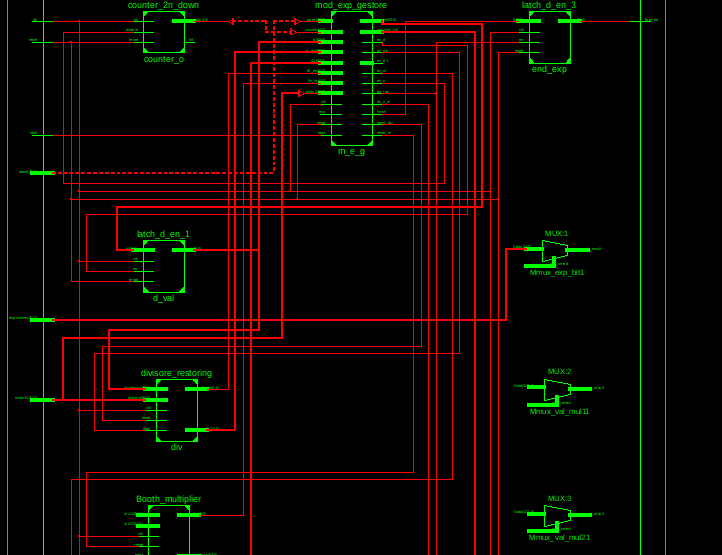
\includegraphics[scale=0.6]{esercizio17/images/exp.png}
	\caption{Hardware Exponentiational}
\end{figure}

Utiliziamo questo algoritmo perch� ci permette di riutilizzare componenti
gi� sviluppati negli esercizi precedenti, difatti osservando lo schematico,
vi � presente un moltiplicatore di Booth e il divisore restoring per
le varie operazioni prodotto e modulo, un contatore down per indicare
quale dei bit dell' esponente dobbiamo analizzare e dei selettori
descritti con il costrutto with select per selezionare quali valori
devono essere moltiplicati. La macchina a stati finiti non fa altro
che eseguire i vari passi dell' algoritmo, per� per problemi relativi
al timing � stata realizzata alla fine con un singolo process, difatti
una prima realizzazione con due process determinava che alcuni registri
contenti i dati dell' operazione assumessero un valore indefinito
(veniva sintetizzata un macchina che doveva avere una frequenza di
clock minore da quella generabile dalla scheda). 

Per problemi di spazio, si � ricorsi a componenti per la moltiplicazione
e divisione seriali, oltre ad riutilizzarli all' interno dello stesso
progetto difatti il moltiplicatore di Booth � stato utilizzato per:
calcolare il prodotto di pq ed l' esponenziazione.

\subsection{Codice}

\href{run:progetti/RSA/RSA.xise}{RSA ISE}

\selectlanguage{italian}%



\selectlanguage{italian}%

\section{Simulazione}

\begin{figure}[H]
	\centering
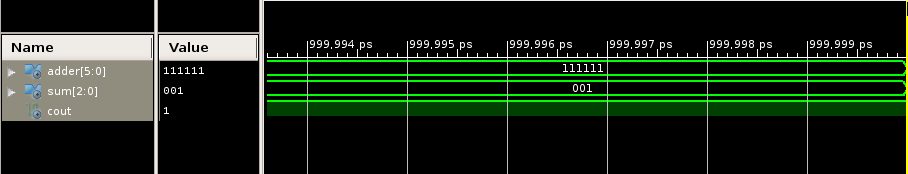
\includegraphics[scale=0.55]{esercizio10/images/carry_save_adder_testbench.png}
	\caption{Carry Save Adder}
\end{figure}\selectlanguage{italian}%



\selectlanguage{italian}%

\section{Sintesi su board FPGA}

Valgono le stesse considerazioni fatte per il Ripple Carry Adder \ref{Sintesi ripple carry},
con la differenza che ci sono sette registri da poter caricare.\selectlanguage{italian}%

\selectlanguage{italian}%



\chapter{Display a 7 segmenti}

\selectlanguage{american}%

\AddToShipoutPicture{\BackgroundPicture{logo.png}{0}}

\selectlanguage{italian}%

\section{Traccia}

Realizzare un dispositivo VHDL che implementa il protocollo UART (a
partire da quello diffuso dalla Digilent). Collegare internamente,
oppure tramite inter- faccia fisica esterna alla board stessa, ad
un\textquoteright altra board oppure ad un PC previo utilizzo di un
physical RS232, due interfacce per trasmette e ricevere ottetti. Svolgere
l\textquoteright esercizio riutilizzando il VHDL messo a disposizione
da Digilent (e disponbile nel materiale del corso) commentando eventuali
ristrutturazioni del codice. (Opzionale) Sviluppare un\textquoteright architettura
per l\textquoteright implementazione del protocollo UART secondo il
paradigma PO/PC ex-novo, evidenziando le similarit`a/dissimilarit`a
con il progetto Digilent.\selectlanguage{italian}%



\selectlanguage{italian}%

\section{Soluzione}


\subsection{Schematici}

Il seguente circuito implementa l' algortimo RSA per la firma di un
messaggio, applica una funzione di hash sul messaggio e verifica che
il messaggio ricevuto sia coretto.

L' intera procedura � divisa nelle seguenti fasi: 
\begin{itemize}
\item vengono scelti i valori caratteristici per inviare il dato (p pari
a 3, q 11, e 7 e d 3) ed il messaggio da inviare;
\item si applica la funzione di hashing sul messaggio, utilizzando il metodo
della moltiplicazione;
\item viene applicata la firma sul messaggio originale utilizzando la chiave
privata, il trasmettitore invia i due dati appena calcolati (anche
se non � presente un vero e proprio invio essendo trasmettitore e
ricevitore implementati sulla stessa board);
\item Il ricevitore applica la chiave pubblica sul messaggio firmato, ne
effettua l' hashing e verifica se la sua versione del messaggio a
cui � stato applicato l' hashing � identico a quello che � stato ricevuto.
\end{itemize}
Cos� facendo garantiamo sia la segretezza( infatti non mandiamo il
messaggio in chiaro), sia l' autenticazione( chi riceve il messaggio
pu� verificare effettuando l' hashing con parametri convenuti non
� stato modificato),

Di seguito vengono descritte le varie componenti che vengono utilizzate
per effettuare l' hashing e firmare il messaggio.

\subsubsection{Funzione hash}

\begin{figure}[H]
	\centering
	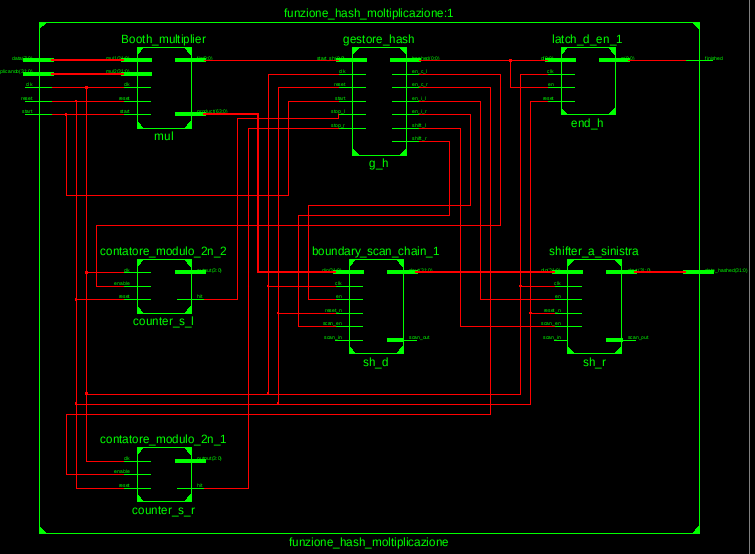
\includegraphics[scale=0.6]{esercizio17/images/hash.png}
	\caption{hasher}
	\label{fig:Mod_exp}
\end{figure}Il circuito � stato realizzato in due differenti modi: 
\begin{itemize}
\item nel primo caso si utilizza una macchina a stati finiti descritta da
cinque stati: 
\begin{itemize}
\item idle, stato di riposo dell' automa; 
\item init in cui si attende che il moltiplicatore termini il suo compito; 
\item shifting\_r in cui il valore della moltiplicazione viene shiftato
a destra; 
\item shifting\_l il valore viene shiftato a sinistra; ended per comunicare
la fine dell' operazione di hash;
\end{itemize}
\item nel secondo si � utilizzato lo stesso procedimento ma il tutto viene
implementato in un process.
\end{itemize}
Viene utilizzata la seconda soluzione perch� occupa meno spazio, dato
che le operazioni di shifting consistono semplicemente, nel caso dello
shifting a destra prendere i sedici bit pi� significativi dal risultato
della moltiplicazione, quando si shifta a sinistra basta accodare
sedici zeri per avere lo stesso risultato della prima soluzione.

Il circito viene cos� descritto poich� tale forma di hashing prevedere
di moltiplicare il dato per un valore A il quale � un numero compreso
tra 0 ed 1, di cui il denominatore � un multiplo di due, per tale
ragione di � scelto di moltiplicare per un valore W ed infine di shiftare
a destra un numero di volte pari al valore dell' esponente, tale numero
� la parte decimale del valore del dato per W (perch� quando shiftiamo
inseriamo degli zero fittizzi), dopodich� si effettua uno shifting
a sinistra di un numero pari di volte affinch� la nostra parte deciamale
rientri nella parte del registro da inviare.

\subsubsection{Esponenziatore}

Per effettuare l' elevazione a potenza con il modulo, ci siamo riferiti
a questo algoritmo :

\begin{figure}[H]
	\centering
	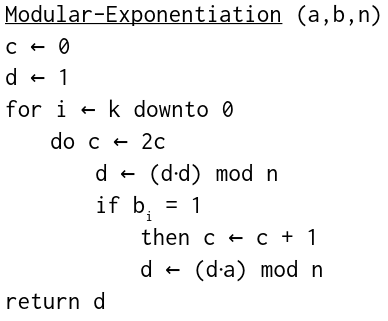
\includegraphics[scale=0.8]{esercizio17/images/mod_exp.png}
	\caption{Algoritmo per modular exponentiational di un messaggio}
	\label{fig:Mod_exp}
\end{figure}

L ' algoritmo cicla sul numero di bit dell ' esponente, moltiplica
il valore d prima per se stesso e ne fa il modulo, questo stesso valore
di d per la base quando il valore dell' esponente in forma binaria
assume valore uno e ne effettua il modulo, (il parametro c non occorre
per il calcolo del valore finale, occorre solo a capire in realt�
alla fine se il numero � stato elevato per il corretto esponente). 

\begin{figure}[H]
	\centering
	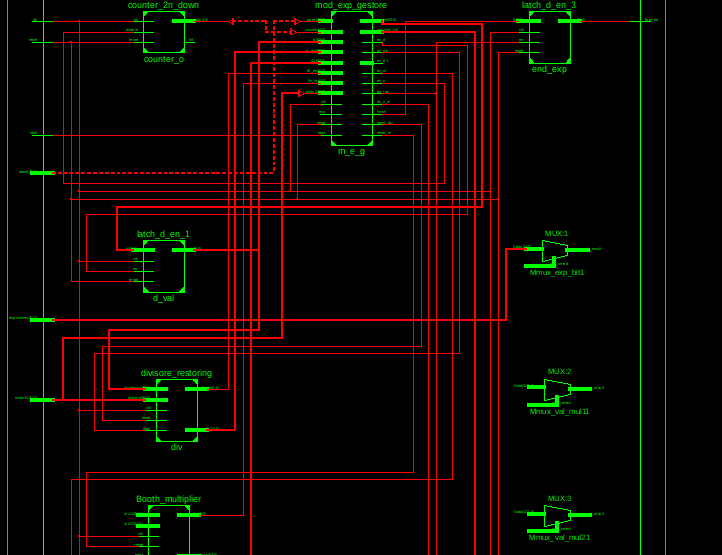
\includegraphics[scale=0.6]{esercizio17/images/exp.png}
	\caption{Hardware Exponentiational}
\end{figure}

Utiliziamo questo algoritmo perch� ci permette di riutilizzare componenti
gi� sviluppati negli esercizi precedenti, difatti osservando lo schematico,
vi � presente un moltiplicatore di Booth e il divisore restoring per
le varie operazioni prodotto e modulo, un contatore down per indicare
quale dei bit dell' esponente dobbiamo analizzare e dei selettori
descritti con il costrutto with select per selezionare quali valori
devono essere moltiplicati. La macchina a stati finiti non fa altro
che eseguire i vari passi dell' algoritmo, per� per problemi relativi
al timing � stata realizzata alla fine con un singolo process, difatti
una prima realizzazione con due process determinava che alcuni registri
contenti i dati dell' operazione assumessero un valore indefinito
(veniva sintetizzata un macchina che doveva avere una frequenza di
clock minore da quella generabile dalla scheda). 

Per problemi di spazio, si � ricorsi a componenti per la moltiplicazione
e divisione seriali, oltre ad riutilizzarli all' interno dello stesso
progetto difatti il moltiplicatore di Booth � stato utilizzato per:
calcolare il prodotto di pq ed l' esponenziazione.

\subsection{Codice}

\href{run:progetti/RSA/RSA.xise}{RSA ISE}

\selectlanguage{italian}%



\selectlanguage{italian}%

\section{Simulazione}

\begin{figure}[H]
	\centering
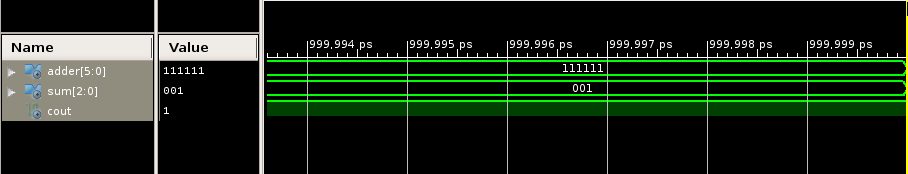
\includegraphics[scale=0.55]{esercizio10/images/carry_save_adder_testbench.png}
	\caption{Carry Save Adder}
\end{figure}\selectlanguage{italian}%



\selectlanguage{italian}%

\section{Sintesi su board FPGA}

Valgono le stesse considerazioni fatte per il Ripple Carry Adder \ref{Sintesi ripple carry},
con la differenza che ci sono sette registri da poter caricare.\selectlanguage{italian}%

\selectlanguage{italian}%



\chapter{Clock Generator}

\selectlanguage{american}%

\AddToShipoutPicture{\BackgroundPicture{logo.png}{0}}

\selectlanguage{italian}%

\section{Traccia}

Realizzare un dispositivo VHDL che implementa il protocollo UART (a
partire da quello diffuso dalla Digilent). Collegare internamente,
oppure tramite inter- faccia fisica esterna alla board stessa, ad
un\textquoteright altra board oppure ad un PC previo utilizzo di un
physical RS232, due interfacce per trasmette e ricevere ottetti. Svolgere
l\textquoteright esercizio riutilizzando il VHDL messo a disposizione
da Digilent (e disponbile nel materiale del corso) commentando eventuali
ristrutturazioni del codice. (Opzionale) Sviluppare un\textquoteright architettura
per l\textquoteright implementazione del protocollo UART secondo il
paradigma PO/PC ex-novo, evidenziando le similarit`a/dissimilarit`a
con il progetto Digilent.\selectlanguage{italian}%



\selectlanguage{italian}%

\section{Soluzione}


\subsection{Schematici}

Il seguente circuito implementa l' algortimo RSA per la firma di un
messaggio, applica una funzione di hash sul messaggio e verifica che
il messaggio ricevuto sia coretto.

L' intera procedura � divisa nelle seguenti fasi: 
\begin{itemize}
\item vengono scelti i valori caratteristici per inviare il dato (p pari
a 3, q 11, e 7 e d 3) ed il messaggio da inviare;
\item si applica la funzione di hashing sul messaggio, utilizzando il metodo
della moltiplicazione;
\item viene applicata la firma sul messaggio originale utilizzando la chiave
privata, il trasmettitore invia i due dati appena calcolati (anche
se non � presente un vero e proprio invio essendo trasmettitore e
ricevitore implementati sulla stessa board);
\item Il ricevitore applica la chiave pubblica sul messaggio firmato, ne
effettua l' hashing e verifica se la sua versione del messaggio a
cui � stato applicato l' hashing � identico a quello che � stato ricevuto.
\end{itemize}
Cos� facendo garantiamo sia la segretezza( infatti non mandiamo il
messaggio in chiaro), sia l' autenticazione( chi riceve il messaggio
pu� verificare effettuando l' hashing con parametri convenuti non
� stato modificato),

Di seguito vengono descritte le varie componenti che vengono utilizzate
per effettuare l' hashing e firmare il messaggio.

\subsubsection{Funzione hash}

\begin{figure}[H]
	\centering
	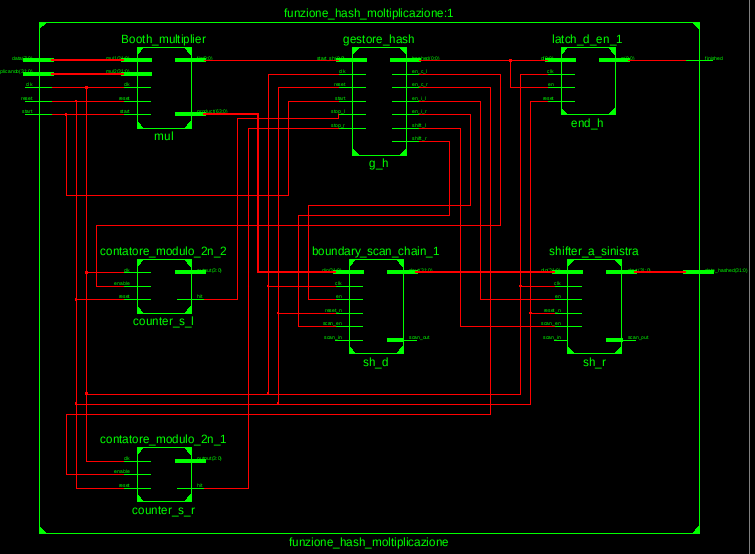
\includegraphics[scale=0.6]{esercizio17/images/hash.png}
	\caption{hasher}
	\label{fig:Mod_exp}
\end{figure}Il circuito � stato realizzato in due differenti modi: 
\begin{itemize}
\item nel primo caso si utilizza una macchina a stati finiti descritta da
cinque stati: 
\begin{itemize}
\item idle, stato di riposo dell' automa; 
\item init in cui si attende che il moltiplicatore termini il suo compito; 
\item shifting\_r in cui il valore della moltiplicazione viene shiftato
a destra; 
\item shifting\_l il valore viene shiftato a sinistra; ended per comunicare
la fine dell' operazione di hash;
\end{itemize}
\item nel secondo si � utilizzato lo stesso procedimento ma il tutto viene
implementato in un process.
\end{itemize}
Viene utilizzata la seconda soluzione perch� occupa meno spazio, dato
che le operazioni di shifting consistono semplicemente, nel caso dello
shifting a destra prendere i sedici bit pi� significativi dal risultato
della moltiplicazione, quando si shifta a sinistra basta accodare
sedici zeri per avere lo stesso risultato della prima soluzione.

Il circito viene cos� descritto poich� tale forma di hashing prevedere
di moltiplicare il dato per un valore A il quale � un numero compreso
tra 0 ed 1, di cui il denominatore � un multiplo di due, per tale
ragione di � scelto di moltiplicare per un valore W ed infine di shiftare
a destra un numero di volte pari al valore dell' esponente, tale numero
� la parte decimale del valore del dato per W (perch� quando shiftiamo
inseriamo degli zero fittizzi), dopodich� si effettua uno shifting
a sinistra di un numero pari di volte affinch� la nostra parte deciamale
rientri nella parte del registro da inviare.

\subsubsection{Esponenziatore}

Per effettuare l' elevazione a potenza con il modulo, ci siamo riferiti
a questo algoritmo :

\begin{figure}[H]
	\centering
	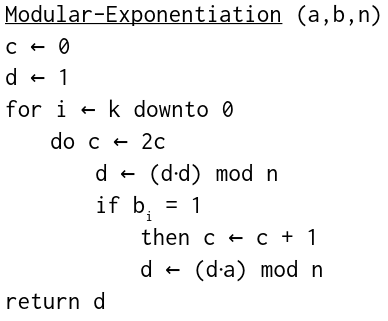
\includegraphics[scale=0.8]{esercizio17/images/mod_exp.png}
	\caption{Algoritmo per modular exponentiational di un messaggio}
	\label{fig:Mod_exp}
\end{figure}

L ' algoritmo cicla sul numero di bit dell ' esponente, moltiplica
il valore d prima per se stesso e ne fa il modulo, questo stesso valore
di d per la base quando il valore dell' esponente in forma binaria
assume valore uno e ne effettua il modulo, (il parametro c non occorre
per il calcolo del valore finale, occorre solo a capire in realt�
alla fine se il numero � stato elevato per il corretto esponente). 

\begin{figure}[H]
	\centering
	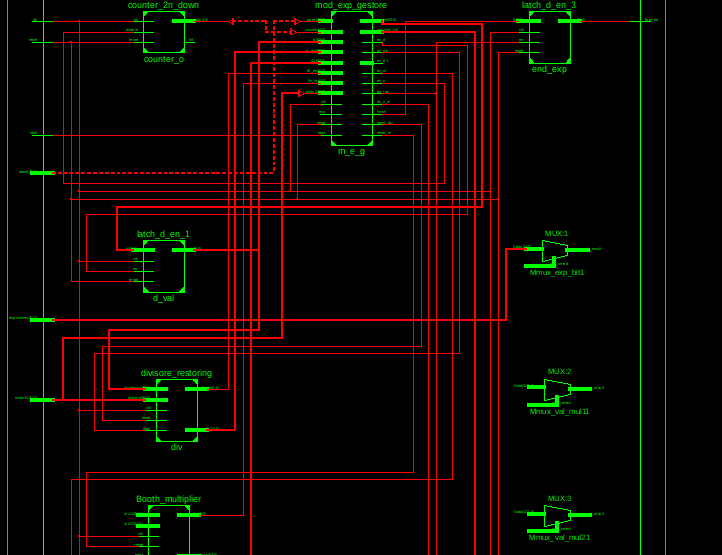
\includegraphics[scale=0.6]{esercizio17/images/exp.png}
	\caption{Hardware Exponentiational}
\end{figure}

Utiliziamo questo algoritmo perch� ci permette di riutilizzare componenti
gi� sviluppati negli esercizi precedenti, difatti osservando lo schematico,
vi � presente un moltiplicatore di Booth e il divisore restoring per
le varie operazioni prodotto e modulo, un contatore down per indicare
quale dei bit dell' esponente dobbiamo analizzare e dei selettori
descritti con il costrutto with select per selezionare quali valori
devono essere moltiplicati. La macchina a stati finiti non fa altro
che eseguire i vari passi dell' algoritmo, per� per problemi relativi
al timing � stata realizzata alla fine con un singolo process, difatti
una prima realizzazione con due process determinava che alcuni registri
contenti i dati dell' operazione assumessero un valore indefinito
(veniva sintetizzata un macchina che doveva avere una frequenza di
clock minore da quella generabile dalla scheda). 

Per problemi di spazio, si � ricorsi a componenti per la moltiplicazione
e divisione seriali, oltre ad riutilizzarli all' interno dello stesso
progetto difatti il moltiplicatore di Booth � stato utilizzato per:
calcolare il prodotto di pq ed l' esponenziazione.

\subsection{Codice}

\href{run:progetti/RSA/RSA.xise}{RSA ISE}

\selectlanguage{italian}%



\selectlanguage{italian}%

\section{Simulazione}

\begin{figure}[H]
	\centering
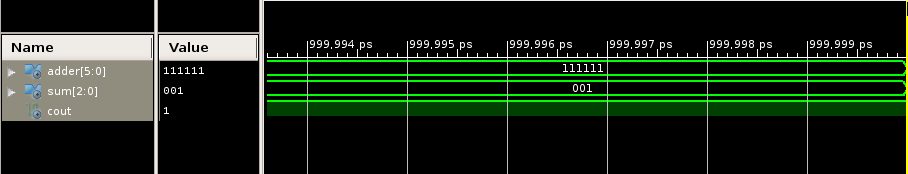
\includegraphics[scale=0.55]{esercizio10/images/carry_save_adder_testbench.png}
	\caption{Carry Save Adder}
\end{figure}\selectlanguage{italian}%



\selectlanguage{italian}%

\section{Sintesi su board FPGA}

Valgono le stesse considerazioni fatte per il Ripple Carry Adder \ref{Sintesi ripple carry},
con la differenza che ci sono sette registri da poter caricare.\selectlanguage{italian}%

\selectlanguage{italian}%



\chapter{Scan Chain}

\selectlanguage{american}%

\AddToShipoutPicture{\BackgroundPicture{logo.png}{0}}

\selectlanguage{italian}%

\section{Traccia}

Realizzare un dispositivo VHDL che implementa il protocollo UART (a
partire da quello diffuso dalla Digilent). Collegare internamente,
oppure tramite inter- faccia fisica esterna alla board stessa, ad
un\textquoteright altra board oppure ad un PC previo utilizzo di un
physical RS232, due interfacce per trasmette e ricevere ottetti. Svolgere
l\textquoteright esercizio riutilizzando il VHDL messo a disposizione
da Digilent (e disponbile nel materiale del corso) commentando eventuali
ristrutturazioni del codice. (Opzionale) Sviluppare un\textquoteright architettura
per l\textquoteright implementazione del protocollo UART secondo il
paradigma PO/PC ex-novo, evidenziando le similarit`a/dissimilarit`a
con il progetto Digilent.\selectlanguage{italian}%



\selectlanguage{italian}%

\section{Soluzione}


\subsection{Schematici}

Il seguente circuito implementa l' algortimo RSA per la firma di un
messaggio, applica una funzione di hash sul messaggio e verifica che
il messaggio ricevuto sia coretto.

L' intera procedura � divisa nelle seguenti fasi: 
\begin{itemize}
\item vengono scelti i valori caratteristici per inviare il dato (p pari
a 3, q 11, e 7 e d 3) ed il messaggio da inviare;
\item si applica la funzione di hashing sul messaggio, utilizzando il metodo
della moltiplicazione;
\item viene applicata la firma sul messaggio originale utilizzando la chiave
privata, il trasmettitore invia i due dati appena calcolati (anche
se non � presente un vero e proprio invio essendo trasmettitore e
ricevitore implementati sulla stessa board);
\item Il ricevitore applica la chiave pubblica sul messaggio firmato, ne
effettua l' hashing e verifica se la sua versione del messaggio a
cui � stato applicato l' hashing � identico a quello che � stato ricevuto.
\end{itemize}
Cos� facendo garantiamo sia la segretezza( infatti non mandiamo il
messaggio in chiaro), sia l' autenticazione( chi riceve il messaggio
pu� verificare effettuando l' hashing con parametri convenuti non
� stato modificato),

Di seguito vengono descritte le varie componenti che vengono utilizzate
per effettuare l' hashing e firmare il messaggio.

\subsubsection{Funzione hash}

\begin{figure}[H]
	\centering
	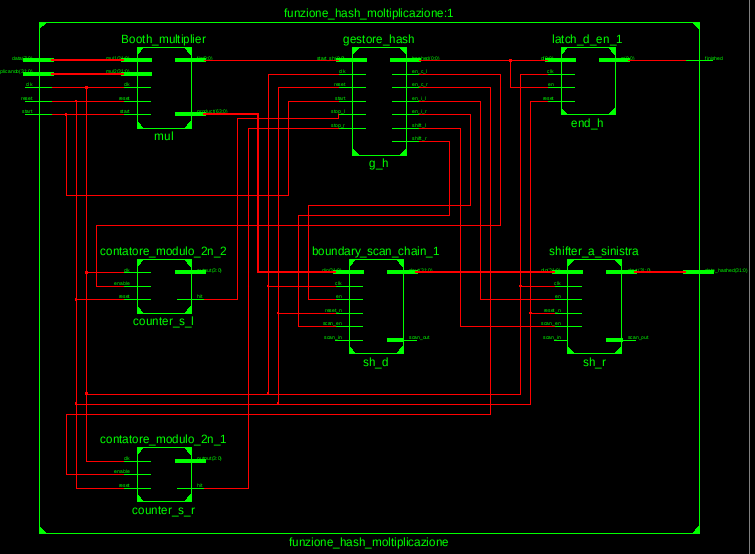
\includegraphics[scale=0.6]{esercizio17/images/hash.png}
	\caption{hasher}
	\label{fig:Mod_exp}
\end{figure}Il circuito � stato realizzato in due differenti modi: 
\begin{itemize}
\item nel primo caso si utilizza una macchina a stati finiti descritta da
cinque stati: 
\begin{itemize}
\item idle, stato di riposo dell' automa; 
\item init in cui si attende che il moltiplicatore termini il suo compito; 
\item shifting\_r in cui il valore della moltiplicazione viene shiftato
a destra; 
\item shifting\_l il valore viene shiftato a sinistra; ended per comunicare
la fine dell' operazione di hash;
\end{itemize}
\item nel secondo si � utilizzato lo stesso procedimento ma il tutto viene
implementato in un process.
\end{itemize}
Viene utilizzata la seconda soluzione perch� occupa meno spazio, dato
che le operazioni di shifting consistono semplicemente, nel caso dello
shifting a destra prendere i sedici bit pi� significativi dal risultato
della moltiplicazione, quando si shifta a sinistra basta accodare
sedici zeri per avere lo stesso risultato della prima soluzione.

Il circito viene cos� descritto poich� tale forma di hashing prevedere
di moltiplicare il dato per un valore A il quale � un numero compreso
tra 0 ed 1, di cui il denominatore � un multiplo di due, per tale
ragione di � scelto di moltiplicare per un valore W ed infine di shiftare
a destra un numero di volte pari al valore dell' esponente, tale numero
� la parte decimale del valore del dato per W (perch� quando shiftiamo
inseriamo degli zero fittizzi), dopodich� si effettua uno shifting
a sinistra di un numero pari di volte affinch� la nostra parte deciamale
rientri nella parte del registro da inviare.

\subsubsection{Esponenziatore}

Per effettuare l' elevazione a potenza con il modulo, ci siamo riferiti
a questo algoritmo :

\begin{figure}[H]
	\centering
	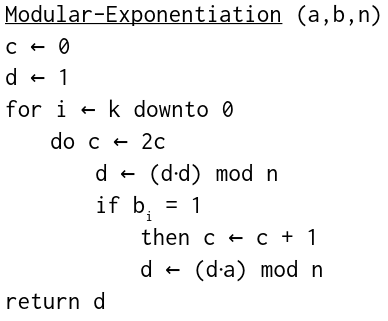
\includegraphics[scale=0.8]{esercizio17/images/mod_exp.png}
	\caption{Algoritmo per modular exponentiational di un messaggio}
	\label{fig:Mod_exp}
\end{figure}

L ' algoritmo cicla sul numero di bit dell ' esponente, moltiplica
il valore d prima per se stesso e ne fa il modulo, questo stesso valore
di d per la base quando il valore dell' esponente in forma binaria
assume valore uno e ne effettua il modulo, (il parametro c non occorre
per il calcolo del valore finale, occorre solo a capire in realt�
alla fine se il numero � stato elevato per il corretto esponente). 

\begin{figure}[H]
	\centering
	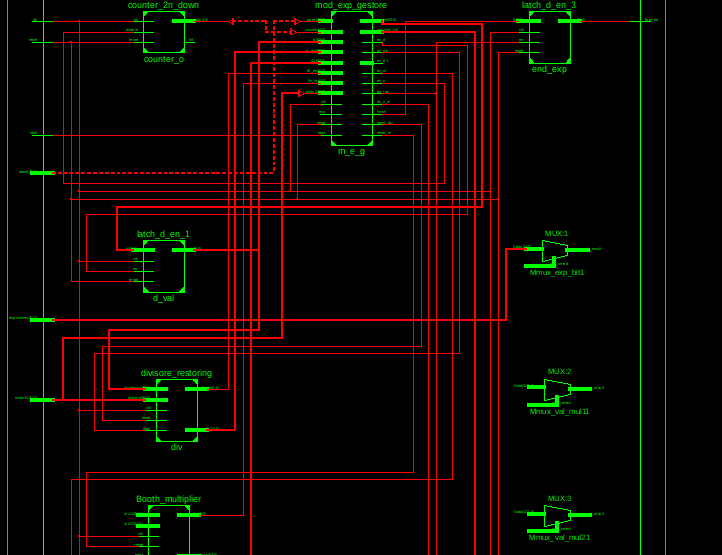
\includegraphics[scale=0.6]{esercizio17/images/exp.png}
	\caption{Hardware Exponentiational}
\end{figure}

Utiliziamo questo algoritmo perch� ci permette di riutilizzare componenti
gi� sviluppati negli esercizi precedenti, difatti osservando lo schematico,
vi � presente un moltiplicatore di Booth e il divisore restoring per
le varie operazioni prodotto e modulo, un contatore down per indicare
quale dei bit dell' esponente dobbiamo analizzare e dei selettori
descritti con il costrutto with select per selezionare quali valori
devono essere moltiplicati. La macchina a stati finiti non fa altro
che eseguire i vari passi dell' algoritmo, per� per problemi relativi
al timing � stata realizzata alla fine con un singolo process, difatti
una prima realizzazione con due process determinava che alcuni registri
contenti i dati dell' operazione assumessero un valore indefinito
(veniva sintetizzata un macchina che doveva avere una frequenza di
clock minore da quella generabile dalla scheda). 

Per problemi di spazio, si � ricorsi a componenti per la moltiplicazione
e divisione seriali, oltre ad riutilizzarli all' interno dello stesso
progetto difatti il moltiplicatore di Booth � stato utilizzato per:
calcolare il prodotto di pq ed l' esponenziazione.

\subsection{Codice}

\href{run:progetti/RSA/RSA.xise}{RSA ISE}

\selectlanguage{italian}%



\selectlanguage{italian}%

\section{Simulazione}

\begin{figure}[H]
	\centering
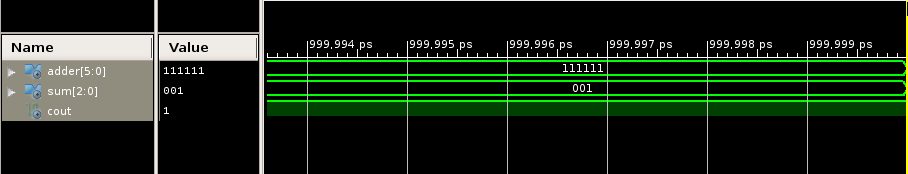
\includegraphics[scale=0.55]{esercizio10/images/carry_save_adder_testbench.png}
	\caption{Carry Save Adder}
\end{figure}\selectlanguage{italian}%



\selectlanguage{italian}%

\section{Sintesi su board FPGA}

Valgono le stesse considerazioni fatte per il Ripple Carry Adder \ref{Sintesi ripple carry},
con la differenza che ci sono sette registri da poter caricare.\selectlanguage{italian}%

\selectlanguage{italian}%



\chapter{Finite State Machine}

\selectlanguage{american}%

\AddToShipoutPicture{\BackgroundPicture{logo.png}{0}}

\selectlanguage{italian}%

\section{Traccia}

Realizzare un dispositivo VHDL che implementa il protocollo UART (a
partire da quello diffuso dalla Digilent). Collegare internamente,
oppure tramite inter- faccia fisica esterna alla board stessa, ad
un\textquoteright altra board oppure ad un PC previo utilizzo di un
physical RS232, due interfacce per trasmette e ricevere ottetti. Svolgere
l\textquoteright esercizio riutilizzando il VHDL messo a disposizione
da Digilent (e disponbile nel materiale del corso) commentando eventuali
ristrutturazioni del codice. (Opzionale) Sviluppare un\textquoteright architettura
per l\textquoteright implementazione del protocollo UART secondo il
paradigma PO/PC ex-novo, evidenziando le similarit`a/dissimilarit`a
con il progetto Digilent.\selectlanguage{italian}%



\selectlanguage{italian}%

\section{Soluzione}


\subsection{Schematici}

Il seguente circuito implementa l' algortimo RSA per la firma di un
messaggio, applica una funzione di hash sul messaggio e verifica che
il messaggio ricevuto sia coretto.

L' intera procedura � divisa nelle seguenti fasi: 
\begin{itemize}
\item vengono scelti i valori caratteristici per inviare il dato (p pari
a 3, q 11, e 7 e d 3) ed il messaggio da inviare;
\item si applica la funzione di hashing sul messaggio, utilizzando il metodo
della moltiplicazione;
\item viene applicata la firma sul messaggio originale utilizzando la chiave
privata, il trasmettitore invia i due dati appena calcolati (anche
se non � presente un vero e proprio invio essendo trasmettitore e
ricevitore implementati sulla stessa board);
\item Il ricevitore applica la chiave pubblica sul messaggio firmato, ne
effettua l' hashing e verifica se la sua versione del messaggio a
cui � stato applicato l' hashing � identico a quello che � stato ricevuto.
\end{itemize}
Cos� facendo garantiamo sia la segretezza( infatti non mandiamo il
messaggio in chiaro), sia l' autenticazione( chi riceve il messaggio
pu� verificare effettuando l' hashing con parametri convenuti non
� stato modificato),

Di seguito vengono descritte le varie componenti che vengono utilizzate
per effettuare l' hashing e firmare il messaggio.

\subsubsection{Funzione hash}

\begin{figure}[H]
	\centering
	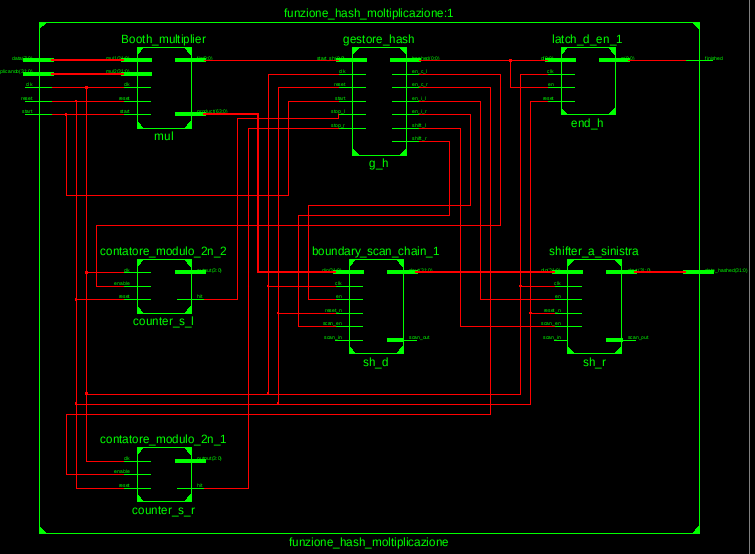
\includegraphics[scale=0.6]{esercizio17/images/hash.png}
	\caption{hasher}
	\label{fig:Mod_exp}
\end{figure}Il circuito � stato realizzato in due differenti modi: 
\begin{itemize}
\item nel primo caso si utilizza una macchina a stati finiti descritta da
cinque stati: 
\begin{itemize}
\item idle, stato di riposo dell' automa; 
\item init in cui si attende che il moltiplicatore termini il suo compito; 
\item shifting\_r in cui il valore della moltiplicazione viene shiftato
a destra; 
\item shifting\_l il valore viene shiftato a sinistra; ended per comunicare
la fine dell' operazione di hash;
\end{itemize}
\item nel secondo si � utilizzato lo stesso procedimento ma il tutto viene
implementato in un process.
\end{itemize}
Viene utilizzata la seconda soluzione perch� occupa meno spazio, dato
che le operazioni di shifting consistono semplicemente, nel caso dello
shifting a destra prendere i sedici bit pi� significativi dal risultato
della moltiplicazione, quando si shifta a sinistra basta accodare
sedici zeri per avere lo stesso risultato della prima soluzione.

Il circito viene cos� descritto poich� tale forma di hashing prevedere
di moltiplicare il dato per un valore A il quale � un numero compreso
tra 0 ed 1, di cui il denominatore � un multiplo di due, per tale
ragione di � scelto di moltiplicare per un valore W ed infine di shiftare
a destra un numero di volte pari al valore dell' esponente, tale numero
� la parte decimale del valore del dato per W (perch� quando shiftiamo
inseriamo degli zero fittizzi), dopodich� si effettua uno shifting
a sinistra di un numero pari di volte affinch� la nostra parte deciamale
rientri nella parte del registro da inviare.

\subsubsection{Esponenziatore}

Per effettuare l' elevazione a potenza con il modulo, ci siamo riferiti
a questo algoritmo :

\begin{figure}[H]
	\centering
	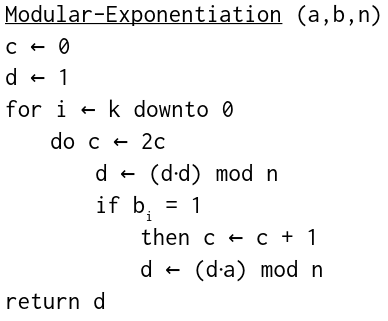
\includegraphics[scale=0.8]{esercizio17/images/mod_exp.png}
	\caption{Algoritmo per modular exponentiational di un messaggio}
	\label{fig:Mod_exp}
\end{figure}

L ' algoritmo cicla sul numero di bit dell ' esponente, moltiplica
il valore d prima per se stesso e ne fa il modulo, questo stesso valore
di d per la base quando il valore dell' esponente in forma binaria
assume valore uno e ne effettua il modulo, (il parametro c non occorre
per il calcolo del valore finale, occorre solo a capire in realt�
alla fine se il numero � stato elevato per il corretto esponente). 

\begin{figure}[H]
	\centering
	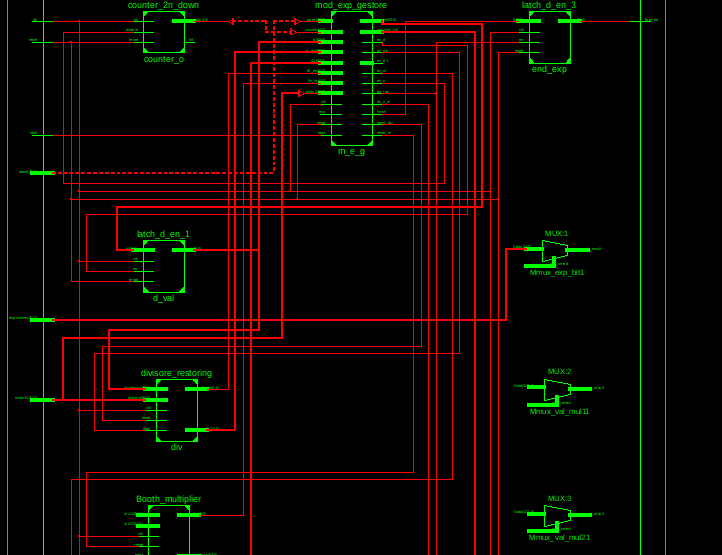
\includegraphics[scale=0.6]{esercizio17/images/exp.png}
	\caption{Hardware Exponentiational}
\end{figure}

Utiliziamo questo algoritmo perch� ci permette di riutilizzare componenti
gi� sviluppati negli esercizi precedenti, difatti osservando lo schematico,
vi � presente un moltiplicatore di Booth e il divisore restoring per
le varie operazioni prodotto e modulo, un contatore down per indicare
quale dei bit dell' esponente dobbiamo analizzare e dei selettori
descritti con il costrutto with select per selezionare quali valori
devono essere moltiplicati. La macchina a stati finiti non fa altro
che eseguire i vari passi dell' algoritmo, per� per problemi relativi
al timing � stata realizzata alla fine con un singolo process, difatti
una prima realizzazione con due process determinava che alcuni registri
contenti i dati dell' operazione assumessero un valore indefinito
(veniva sintetizzata un macchina che doveva avere una frequenza di
clock minore da quella generabile dalla scheda). 

Per problemi di spazio, si � ricorsi a componenti per la moltiplicazione
e divisione seriali, oltre ad riutilizzarli all' interno dello stesso
progetto difatti il moltiplicatore di Booth � stato utilizzato per:
calcolare il prodotto di pq ed l' esponenziazione.

\subsection{Codice}

\href{run:progetti/RSA/RSA.xise}{RSA ISE}

\selectlanguage{italian}%



\selectlanguage{italian}%

\section{Simulazione}

\begin{figure}[H]
	\centering
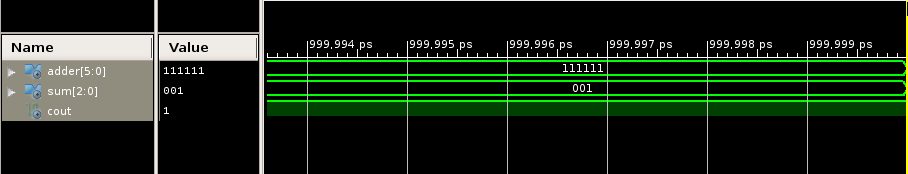
\includegraphics[scale=0.55]{esercizio10/images/carry_save_adder_testbench.png}
	\caption{Carry Save Adder}
\end{figure}\selectlanguage{italian}%



\selectlanguage{italian}%

\section{Sintesi su board FPGA}

Valgono le stesse considerazioni fatte per il Ripple Carry Adder \ref{Sintesi ripple carry},
con la differenza che ci sono sette registri da poter caricare.\selectlanguage{italian}%

\selectlanguage{italian}%



\chapter{Ripple Carry}

\selectlanguage{american}%

\AddToShipoutPicture{\BackgroundPicture{logo.png}{0}}

\selectlanguage{italian}%

\section{Traccia}

Realizzare un dispositivo VHDL che implementa il protocollo UART (a
partire da quello diffuso dalla Digilent). Collegare internamente,
oppure tramite inter- faccia fisica esterna alla board stessa, ad
un\textquoteright altra board oppure ad un PC previo utilizzo di un
physical RS232, due interfacce per trasmette e ricevere ottetti. Svolgere
l\textquoteright esercizio riutilizzando il VHDL messo a disposizione
da Digilent (e disponbile nel materiale del corso) commentando eventuali
ristrutturazioni del codice. (Opzionale) Sviluppare un\textquoteright architettura
per l\textquoteright implementazione del protocollo UART secondo il
paradigma PO/PC ex-novo, evidenziando le similarit`a/dissimilarit`a
con il progetto Digilent.\selectlanguage{italian}%



\selectlanguage{italian}%

\section{Soluzione}


\subsection{Schematici}

Il seguente circuito implementa l' algortimo RSA per la firma di un
messaggio, applica una funzione di hash sul messaggio e verifica che
il messaggio ricevuto sia coretto.

L' intera procedura � divisa nelle seguenti fasi: 
\begin{itemize}
\item vengono scelti i valori caratteristici per inviare il dato (p pari
a 3, q 11, e 7 e d 3) ed il messaggio da inviare;
\item si applica la funzione di hashing sul messaggio, utilizzando il metodo
della moltiplicazione;
\item viene applicata la firma sul messaggio originale utilizzando la chiave
privata, il trasmettitore invia i due dati appena calcolati (anche
se non � presente un vero e proprio invio essendo trasmettitore e
ricevitore implementati sulla stessa board);
\item Il ricevitore applica la chiave pubblica sul messaggio firmato, ne
effettua l' hashing e verifica se la sua versione del messaggio a
cui � stato applicato l' hashing � identico a quello che � stato ricevuto.
\end{itemize}
Cos� facendo garantiamo sia la segretezza( infatti non mandiamo il
messaggio in chiaro), sia l' autenticazione( chi riceve il messaggio
pu� verificare effettuando l' hashing con parametri convenuti non
� stato modificato),

Di seguito vengono descritte le varie componenti che vengono utilizzate
per effettuare l' hashing e firmare il messaggio.

\subsubsection{Funzione hash}

\begin{figure}[H]
	\centering
	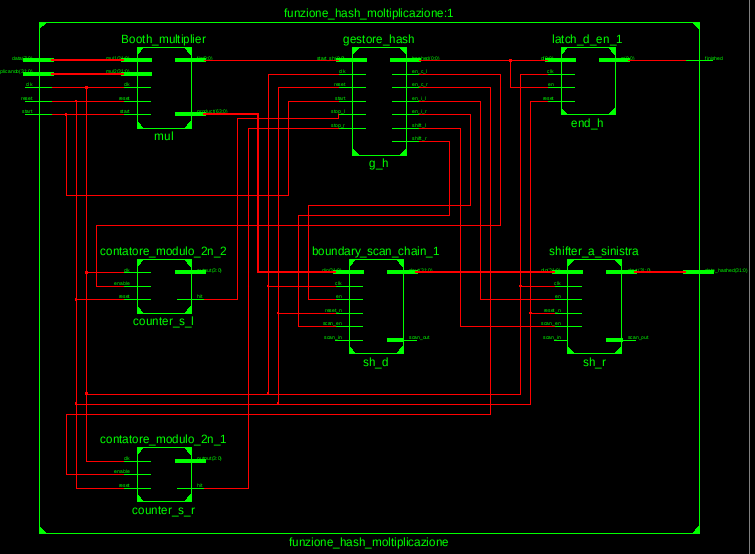
\includegraphics[scale=0.6]{esercizio17/images/hash.png}
	\caption{hasher}
	\label{fig:Mod_exp}
\end{figure}Il circuito � stato realizzato in due differenti modi: 
\begin{itemize}
\item nel primo caso si utilizza una macchina a stati finiti descritta da
cinque stati: 
\begin{itemize}
\item idle, stato di riposo dell' automa; 
\item init in cui si attende che il moltiplicatore termini il suo compito; 
\item shifting\_r in cui il valore della moltiplicazione viene shiftato
a destra; 
\item shifting\_l il valore viene shiftato a sinistra; ended per comunicare
la fine dell' operazione di hash;
\end{itemize}
\item nel secondo si � utilizzato lo stesso procedimento ma il tutto viene
implementato in un process.
\end{itemize}
Viene utilizzata la seconda soluzione perch� occupa meno spazio, dato
che le operazioni di shifting consistono semplicemente, nel caso dello
shifting a destra prendere i sedici bit pi� significativi dal risultato
della moltiplicazione, quando si shifta a sinistra basta accodare
sedici zeri per avere lo stesso risultato della prima soluzione.

Il circito viene cos� descritto poich� tale forma di hashing prevedere
di moltiplicare il dato per un valore A il quale � un numero compreso
tra 0 ed 1, di cui il denominatore � un multiplo di due, per tale
ragione di � scelto di moltiplicare per un valore W ed infine di shiftare
a destra un numero di volte pari al valore dell' esponente, tale numero
� la parte decimale del valore del dato per W (perch� quando shiftiamo
inseriamo degli zero fittizzi), dopodich� si effettua uno shifting
a sinistra di un numero pari di volte affinch� la nostra parte deciamale
rientri nella parte del registro da inviare.

\subsubsection{Esponenziatore}

Per effettuare l' elevazione a potenza con il modulo, ci siamo riferiti
a questo algoritmo :

\begin{figure}[H]
	\centering
	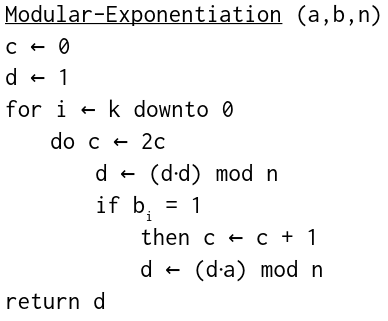
\includegraphics[scale=0.8]{esercizio17/images/mod_exp.png}
	\caption{Algoritmo per modular exponentiational di un messaggio}
	\label{fig:Mod_exp}
\end{figure}

L ' algoritmo cicla sul numero di bit dell ' esponente, moltiplica
il valore d prima per se stesso e ne fa il modulo, questo stesso valore
di d per la base quando il valore dell' esponente in forma binaria
assume valore uno e ne effettua il modulo, (il parametro c non occorre
per il calcolo del valore finale, occorre solo a capire in realt�
alla fine se il numero � stato elevato per il corretto esponente). 

\begin{figure}[H]
	\centering
	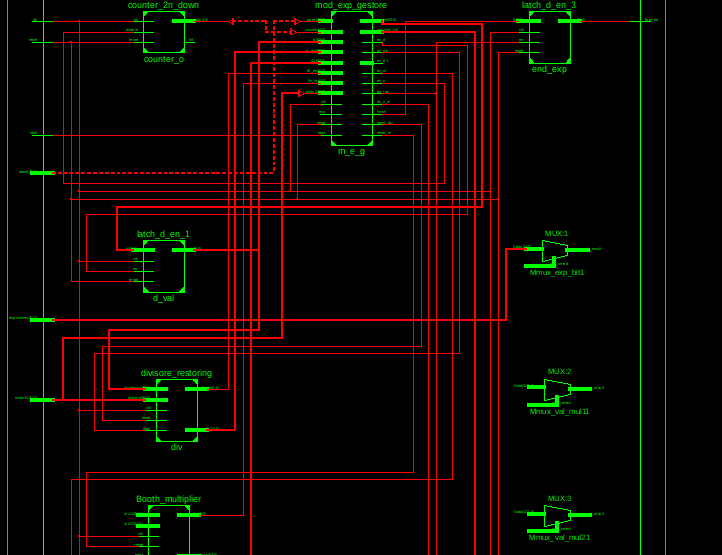
\includegraphics[scale=0.6]{esercizio17/images/exp.png}
	\caption{Hardware Exponentiational}
\end{figure}

Utiliziamo questo algoritmo perch� ci permette di riutilizzare componenti
gi� sviluppati negli esercizi precedenti, difatti osservando lo schematico,
vi � presente un moltiplicatore di Booth e il divisore restoring per
le varie operazioni prodotto e modulo, un contatore down per indicare
quale dei bit dell' esponente dobbiamo analizzare e dei selettori
descritti con il costrutto with select per selezionare quali valori
devono essere moltiplicati. La macchina a stati finiti non fa altro
che eseguire i vari passi dell' algoritmo, per� per problemi relativi
al timing � stata realizzata alla fine con un singolo process, difatti
una prima realizzazione con due process determinava che alcuni registri
contenti i dati dell' operazione assumessero un valore indefinito
(veniva sintetizzata un macchina che doveva avere una frequenza di
clock minore da quella generabile dalla scheda). 

Per problemi di spazio, si � ricorsi a componenti per la moltiplicazione
e divisione seriali, oltre ad riutilizzarli all' interno dello stesso
progetto difatti il moltiplicatore di Booth � stato utilizzato per:
calcolare il prodotto di pq ed l' esponenziazione.

\subsection{Codice}

\href{run:progetti/RSA/RSA.xise}{RSA ISE}

\selectlanguage{italian}%



\selectlanguage{italian}%

\section{Simulazione}

\begin{figure}[H]
	\centering
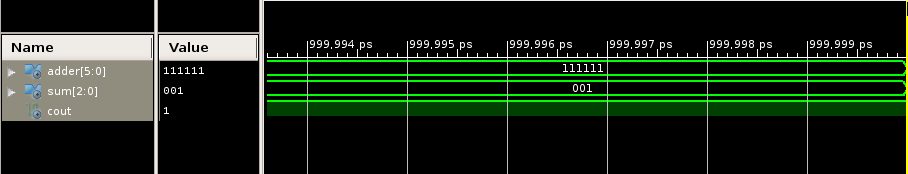
\includegraphics[scale=0.55]{esercizio10/images/carry_save_adder_testbench.png}
	\caption{Carry Save Adder}
\end{figure}\selectlanguage{italian}%



\selectlanguage{italian}%

\section{Sintesi su board FPGA}

Valgono le stesse considerazioni fatte per il Ripple Carry Adder \ref{Sintesi ripple carry},
con la differenza che ci sono sette registri da poter caricare.\selectlanguage{italian}%

\selectlanguage{italian}%



\chapter{Carry Look Ahead}

\selectlanguage{american}%

\AddToShipoutPicture{\BackgroundPicture{logo.png}{0}}

\selectlanguage{italian}%

\section{Traccia}

Realizzare un dispositivo VHDL che implementa il protocollo UART (a
partire da quello diffuso dalla Digilent). Collegare internamente,
oppure tramite inter- faccia fisica esterna alla board stessa, ad
un\textquoteright altra board oppure ad un PC previo utilizzo di un
physical RS232, due interfacce per trasmette e ricevere ottetti. Svolgere
l\textquoteright esercizio riutilizzando il VHDL messo a disposizione
da Digilent (e disponbile nel materiale del corso) commentando eventuali
ristrutturazioni del codice. (Opzionale) Sviluppare un\textquoteright architettura
per l\textquoteright implementazione del protocollo UART secondo il
paradigma PO/PC ex-novo, evidenziando le similarit`a/dissimilarit`a
con il progetto Digilent.\selectlanguage{italian}%



\selectlanguage{italian}%

\section{Soluzione}


\subsection{Schematici}

Il seguente circuito implementa l' algortimo RSA per la firma di un
messaggio, applica una funzione di hash sul messaggio e verifica che
il messaggio ricevuto sia coretto.

L' intera procedura � divisa nelle seguenti fasi: 
\begin{itemize}
\item vengono scelti i valori caratteristici per inviare il dato (p pari
a 3, q 11, e 7 e d 3) ed il messaggio da inviare;
\item si applica la funzione di hashing sul messaggio, utilizzando il metodo
della moltiplicazione;
\item viene applicata la firma sul messaggio originale utilizzando la chiave
privata, il trasmettitore invia i due dati appena calcolati (anche
se non � presente un vero e proprio invio essendo trasmettitore e
ricevitore implementati sulla stessa board);
\item Il ricevitore applica la chiave pubblica sul messaggio firmato, ne
effettua l' hashing e verifica se la sua versione del messaggio a
cui � stato applicato l' hashing � identico a quello che � stato ricevuto.
\end{itemize}
Cos� facendo garantiamo sia la segretezza( infatti non mandiamo il
messaggio in chiaro), sia l' autenticazione( chi riceve il messaggio
pu� verificare effettuando l' hashing con parametri convenuti non
� stato modificato),

Di seguito vengono descritte le varie componenti che vengono utilizzate
per effettuare l' hashing e firmare il messaggio.

\subsubsection{Funzione hash}

\begin{figure}[H]
	\centering
	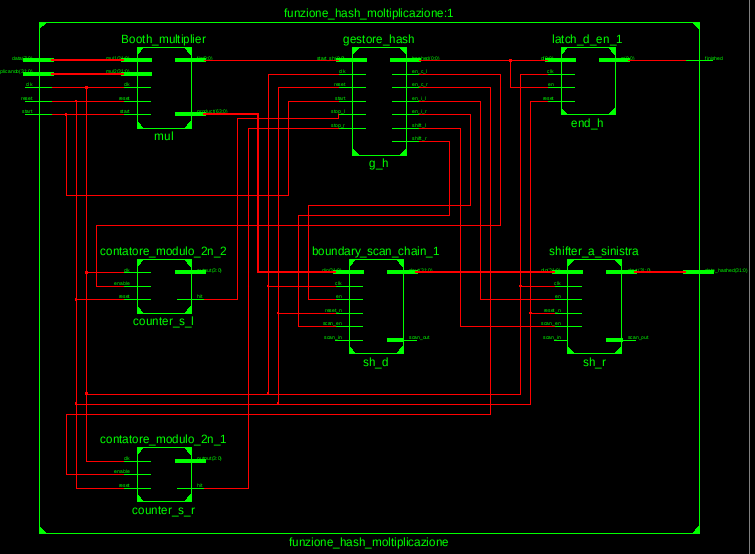
\includegraphics[scale=0.6]{esercizio17/images/hash.png}
	\caption{hasher}
	\label{fig:Mod_exp}
\end{figure}Il circuito � stato realizzato in due differenti modi: 
\begin{itemize}
\item nel primo caso si utilizza una macchina a stati finiti descritta da
cinque stati: 
\begin{itemize}
\item idle, stato di riposo dell' automa; 
\item init in cui si attende che il moltiplicatore termini il suo compito; 
\item shifting\_r in cui il valore della moltiplicazione viene shiftato
a destra; 
\item shifting\_l il valore viene shiftato a sinistra; ended per comunicare
la fine dell' operazione di hash;
\end{itemize}
\item nel secondo si � utilizzato lo stesso procedimento ma il tutto viene
implementato in un process.
\end{itemize}
Viene utilizzata la seconda soluzione perch� occupa meno spazio, dato
che le operazioni di shifting consistono semplicemente, nel caso dello
shifting a destra prendere i sedici bit pi� significativi dal risultato
della moltiplicazione, quando si shifta a sinistra basta accodare
sedici zeri per avere lo stesso risultato della prima soluzione.

Il circito viene cos� descritto poich� tale forma di hashing prevedere
di moltiplicare il dato per un valore A il quale � un numero compreso
tra 0 ed 1, di cui il denominatore � un multiplo di due, per tale
ragione di � scelto di moltiplicare per un valore W ed infine di shiftare
a destra un numero di volte pari al valore dell' esponente, tale numero
� la parte decimale del valore del dato per W (perch� quando shiftiamo
inseriamo degli zero fittizzi), dopodich� si effettua uno shifting
a sinistra di un numero pari di volte affinch� la nostra parte deciamale
rientri nella parte del registro da inviare.

\subsubsection{Esponenziatore}

Per effettuare l' elevazione a potenza con il modulo, ci siamo riferiti
a questo algoritmo :

\begin{figure}[H]
	\centering
	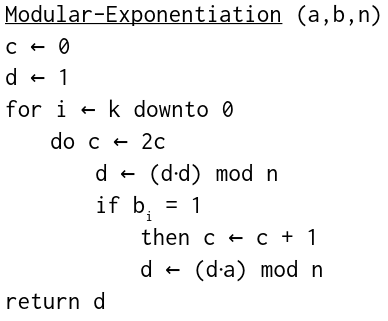
\includegraphics[scale=0.8]{esercizio17/images/mod_exp.png}
	\caption{Algoritmo per modular exponentiational di un messaggio}
	\label{fig:Mod_exp}
\end{figure}

L ' algoritmo cicla sul numero di bit dell ' esponente, moltiplica
il valore d prima per se stesso e ne fa il modulo, questo stesso valore
di d per la base quando il valore dell' esponente in forma binaria
assume valore uno e ne effettua il modulo, (il parametro c non occorre
per il calcolo del valore finale, occorre solo a capire in realt�
alla fine se il numero � stato elevato per il corretto esponente). 

\begin{figure}[H]
	\centering
	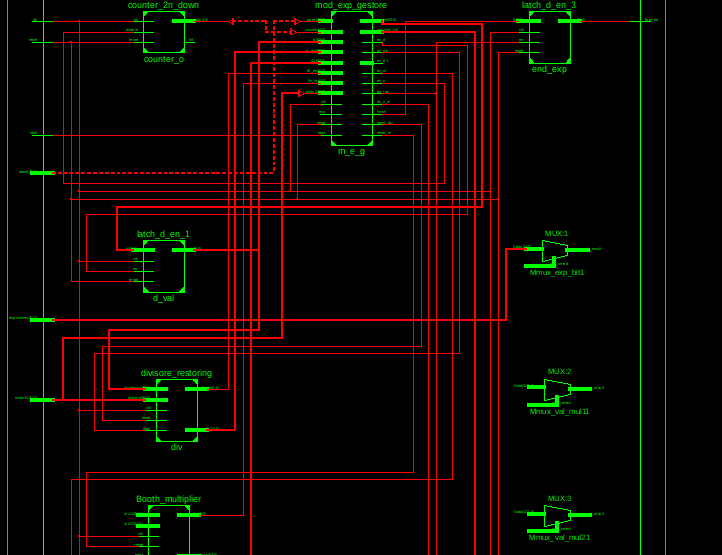
\includegraphics[scale=0.6]{esercizio17/images/exp.png}
	\caption{Hardware Exponentiational}
\end{figure}

Utiliziamo questo algoritmo perch� ci permette di riutilizzare componenti
gi� sviluppati negli esercizi precedenti, difatti osservando lo schematico,
vi � presente un moltiplicatore di Booth e il divisore restoring per
le varie operazioni prodotto e modulo, un contatore down per indicare
quale dei bit dell' esponente dobbiamo analizzare e dei selettori
descritti con il costrutto with select per selezionare quali valori
devono essere moltiplicati. La macchina a stati finiti non fa altro
che eseguire i vari passi dell' algoritmo, per� per problemi relativi
al timing � stata realizzata alla fine con un singolo process, difatti
una prima realizzazione con due process determinava che alcuni registri
contenti i dati dell' operazione assumessero un valore indefinito
(veniva sintetizzata un macchina che doveva avere una frequenza di
clock minore da quella generabile dalla scheda). 

Per problemi di spazio, si � ricorsi a componenti per la moltiplicazione
e divisione seriali, oltre ad riutilizzarli all' interno dello stesso
progetto difatti il moltiplicatore di Booth � stato utilizzato per:
calcolare il prodotto di pq ed l' esponenziazione.

\subsection{Codice}

\href{run:progetti/RSA/RSA.xise}{RSA ISE}

\selectlanguage{italian}%



\selectlanguage{italian}%

\section{Simulazione}

\begin{figure}[H]
	\centering
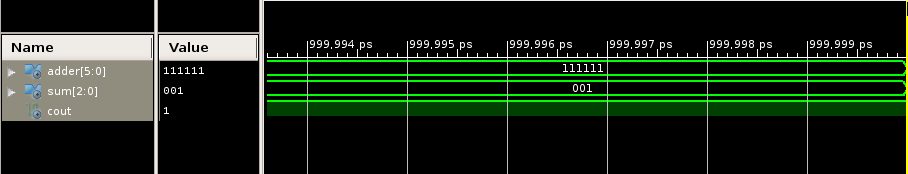
\includegraphics[scale=0.55]{esercizio10/images/carry_save_adder_testbench.png}
	\caption{Carry Save Adder}
\end{figure}\selectlanguage{italian}%



\selectlanguage{italian}%

\section{Sintesi su board FPGA}

Valgono le stesse considerazioni fatte per il Ripple Carry Adder \ref{Sintesi ripple carry},
con la differenza che ci sono sette registri da poter caricare.\selectlanguage{italian}%

\selectlanguage{italian}%



\chapter{Carry Save}

\selectlanguage{american}%

\AddToShipoutPicture{\BackgroundPicture{logo.png}{0}}

\selectlanguage{italian}%

\section{Traccia}

Realizzare un dispositivo VHDL che implementa il protocollo UART (a
partire da quello diffuso dalla Digilent). Collegare internamente,
oppure tramite inter- faccia fisica esterna alla board stessa, ad
un\textquoteright altra board oppure ad un PC previo utilizzo di un
physical RS232, due interfacce per trasmette e ricevere ottetti. Svolgere
l\textquoteright esercizio riutilizzando il VHDL messo a disposizione
da Digilent (e disponbile nel materiale del corso) commentando eventuali
ristrutturazioni del codice. (Opzionale) Sviluppare un\textquoteright architettura
per l\textquoteright implementazione del protocollo UART secondo il
paradigma PO/PC ex-novo, evidenziando le similarit`a/dissimilarit`a
con il progetto Digilent.\selectlanguage{italian}%



\selectlanguage{italian}%

\section{Soluzione}


\subsection{Schematici}

Il seguente circuito implementa l' algortimo RSA per la firma di un
messaggio, applica una funzione di hash sul messaggio e verifica che
il messaggio ricevuto sia coretto.

L' intera procedura � divisa nelle seguenti fasi: 
\begin{itemize}
\item vengono scelti i valori caratteristici per inviare il dato (p pari
a 3, q 11, e 7 e d 3) ed il messaggio da inviare;
\item si applica la funzione di hashing sul messaggio, utilizzando il metodo
della moltiplicazione;
\item viene applicata la firma sul messaggio originale utilizzando la chiave
privata, il trasmettitore invia i due dati appena calcolati (anche
se non � presente un vero e proprio invio essendo trasmettitore e
ricevitore implementati sulla stessa board);
\item Il ricevitore applica la chiave pubblica sul messaggio firmato, ne
effettua l' hashing e verifica se la sua versione del messaggio a
cui � stato applicato l' hashing � identico a quello che � stato ricevuto.
\end{itemize}
Cos� facendo garantiamo sia la segretezza( infatti non mandiamo il
messaggio in chiaro), sia l' autenticazione( chi riceve il messaggio
pu� verificare effettuando l' hashing con parametri convenuti non
� stato modificato),

Di seguito vengono descritte le varie componenti che vengono utilizzate
per effettuare l' hashing e firmare il messaggio.

\subsubsection{Funzione hash}

\begin{figure}[H]
	\centering
	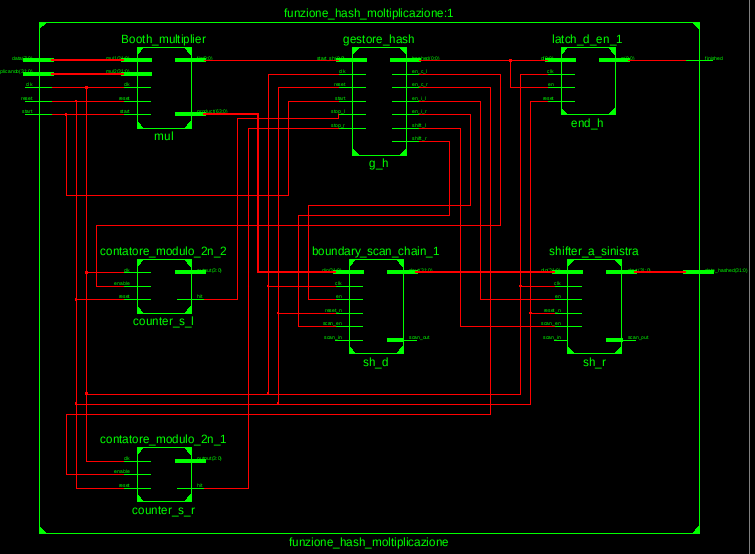
\includegraphics[scale=0.6]{esercizio17/images/hash.png}
	\caption{hasher}
	\label{fig:Mod_exp}
\end{figure}Il circuito � stato realizzato in due differenti modi: 
\begin{itemize}
\item nel primo caso si utilizza una macchina a stati finiti descritta da
cinque stati: 
\begin{itemize}
\item idle, stato di riposo dell' automa; 
\item init in cui si attende che il moltiplicatore termini il suo compito; 
\item shifting\_r in cui il valore della moltiplicazione viene shiftato
a destra; 
\item shifting\_l il valore viene shiftato a sinistra; ended per comunicare
la fine dell' operazione di hash;
\end{itemize}
\item nel secondo si � utilizzato lo stesso procedimento ma il tutto viene
implementato in un process.
\end{itemize}
Viene utilizzata la seconda soluzione perch� occupa meno spazio, dato
che le operazioni di shifting consistono semplicemente, nel caso dello
shifting a destra prendere i sedici bit pi� significativi dal risultato
della moltiplicazione, quando si shifta a sinistra basta accodare
sedici zeri per avere lo stesso risultato della prima soluzione.

Il circito viene cos� descritto poich� tale forma di hashing prevedere
di moltiplicare il dato per un valore A il quale � un numero compreso
tra 0 ed 1, di cui il denominatore � un multiplo di due, per tale
ragione di � scelto di moltiplicare per un valore W ed infine di shiftare
a destra un numero di volte pari al valore dell' esponente, tale numero
� la parte decimale del valore del dato per W (perch� quando shiftiamo
inseriamo degli zero fittizzi), dopodich� si effettua uno shifting
a sinistra di un numero pari di volte affinch� la nostra parte deciamale
rientri nella parte del registro da inviare.

\subsubsection{Esponenziatore}

Per effettuare l' elevazione a potenza con il modulo, ci siamo riferiti
a questo algoritmo :

\begin{figure}[H]
	\centering
	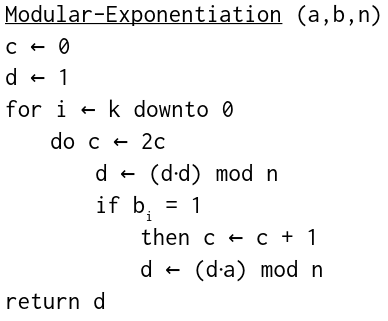
\includegraphics[scale=0.8]{esercizio17/images/mod_exp.png}
	\caption{Algoritmo per modular exponentiational di un messaggio}
	\label{fig:Mod_exp}
\end{figure}

L ' algoritmo cicla sul numero di bit dell ' esponente, moltiplica
il valore d prima per se stesso e ne fa il modulo, questo stesso valore
di d per la base quando il valore dell' esponente in forma binaria
assume valore uno e ne effettua il modulo, (il parametro c non occorre
per il calcolo del valore finale, occorre solo a capire in realt�
alla fine se il numero � stato elevato per il corretto esponente). 

\begin{figure}[H]
	\centering
	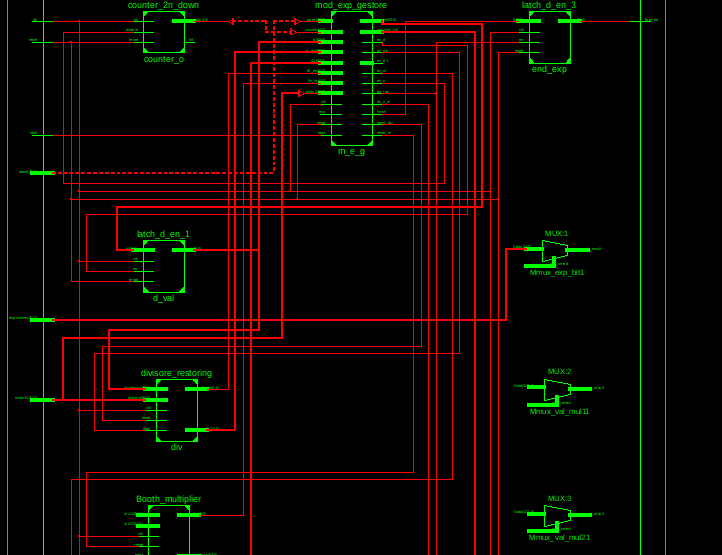
\includegraphics[scale=0.6]{esercizio17/images/exp.png}
	\caption{Hardware Exponentiational}
\end{figure}

Utiliziamo questo algoritmo perch� ci permette di riutilizzare componenti
gi� sviluppati negli esercizi precedenti, difatti osservando lo schematico,
vi � presente un moltiplicatore di Booth e il divisore restoring per
le varie operazioni prodotto e modulo, un contatore down per indicare
quale dei bit dell' esponente dobbiamo analizzare e dei selettori
descritti con il costrutto with select per selezionare quali valori
devono essere moltiplicati. La macchina a stati finiti non fa altro
che eseguire i vari passi dell' algoritmo, per� per problemi relativi
al timing � stata realizzata alla fine con un singolo process, difatti
una prima realizzazione con due process determinava che alcuni registri
contenti i dati dell' operazione assumessero un valore indefinito
(veniva sintetizzata un macchina che doveva avere una frequenza di
clock minore da quella generabile dalla scheda). 

Per problemi di spazio, si � ricorsi a componenti per la moltiplicazione
e divisione seriali, oltre ad riutilizzarli all' interno dello stesso
progetto difatti il moltiplicatore di Booth � stato utilizzato per:
calcolare il prodotto di pq ed l' esponenziazione.

\subsection{Codice}

\href{run:progetti/RSA/RSA.xise}{RSA ISE}

\selectlanguage{italian}%



\selectlanguage{italian}%

\section{Simulazione}

\begin{figure}[H]
	\centering
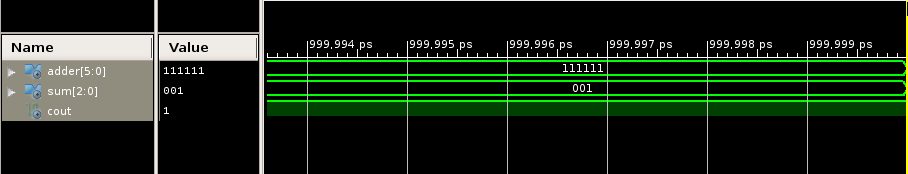
\includegraphics[scale=0.55]{esercizio10/images/carry_save_adder_testbench.png}
	\caption{Carry Save Adder}
\end{figure}\selectlanguage{italian}%



\selectlanguage{italian}%

\section{Sintesi su board FPGA}

Valgono le stesse considerazioni fatte per il Ripple Carry Adder \ref{Sintesi ripple carry},
con la differenza che ci sono sette registri da poter caricare.\selectlanguage{italian}%

\selectlanguage{italian}%



\chapter{Carry Select}

\selectlanguage{american}%

\AddToShipoutPicture{\BackgroundPicture{logo.png}{0}}

\selectlanguage{italian}%

\section{Traccia}

Realizzare un dispositivo VHDL che implementa il protocollo UART (a
partire da quello diffuso dalla Digilent). Collegare internamente,
oppure tramite inter- faccia fisica esterna alla board stessa, ad
un\textquoteright altra board oppure ad un PC previo utilizzo di un
physical RS232, due interfacce per trasmette e ricevere ottetti. Svolgere
l\textquoteright esercizio riutilizzando il VHDL messo a disposizione
da Digilent (e disponbile nel materiale del corso) commentando eventuali
ristrutturazioni del codice. (Opzionale) Sviluppare un\textquoteright architettura
per l\textquoteright implementazione del protocollo UART secondo il
paradigma PO/PC ex-novo, evidenziando le similarit`a/dissimilarit`a
con il progetto Digilent.\selectlanguage{italian}%



\selectlanguage{italian}%

\section{Soluzione}


\subsection{Schematici}

Il seguente circuito implementa l' algortimo RSA per la firma di un
messaggio, applica una funzione di hash sul messaggio e verifica che
il messaggio ricevuto sia coretto.

L' intera procedura � divisa nelle seguenti fasi: 
\begin{itemize}
\item vengono scelti i valori caratteristici per inviare il dato (p pari
a 3, q 11, e 7 e d 3) ed il messaggio da inviare;
\item si applica la funzione di hashing sul messaggio, utilizzando il metodo
della moltiplicazione;
\item viene applicata la firma sul messaggio originale utilizzando la chiave
privata, il trasmettitore invia i due dati appena calcolati (anche
se non � presente un vero e proprio invio essendo trasmettitore e
ricevitore implementati sulla stessa board);
\item Il ricevitore applica la chiave pubblica sul messaggio firmato, ne
effettua l' hashing e verifica se la sua versione del messaggio a
cui � stato applicato l' hashing � identico a quello che � stato ricevuto.
\end{itemize}
Cos� facendo garantiamo sia la segretezza( infatti non mandiamo il
messaggio in chiaro), sia l' autenticazione( chi riceve il messaggio
pu� verificare effettuando l' hashing con parametri convenuti non
� stato modificato),

Di seguito vengono descritte le varie componenti che vengono utilizzate
per effettuare l' hashing e firmare il messaggio.

\subsubsection{Funzione hash}

\begin{figure}[H]
	\centering
	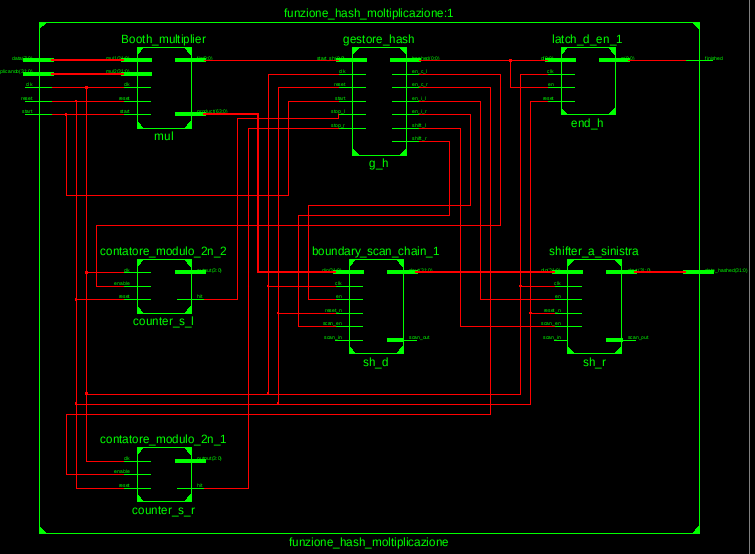
\includegraphics[scale=0.6]{esercizio17/images/hash.png}
	\caption{hasher}
	\label{fig:Mod_exp}
\end{figure}Il circuito � stato realizzato in due differenti modi: 
\begin{itemize}
\item nel primo caso si utilizza una macchina a stati finiti descritta da
cinque stati: 
\begin{itemize}
\item idle, stato di riposo dell' automa; 
\item init in cui si attende che il moltiplicatore termini il suo compito; 
\item shifting\_r in cui il valore della moltiplicazione viene shiftato
a destra; 
\item shifting\_l il valore viene shiftato a sinistra; ended per comunicare
la fine dell' operazione di hash;
\end{itemize}
\item nel secondo si � utilizzato lo stesso procedimento ma il tutto viene
implementato in un process.
\end{itemize}
Viene utilizzata la seconda soluzione perch� occupa meno spazio, dato
che le operazioni di shifting consistono semplicemente, nel caso dello
shifting a destra prendere i sedici bit pi� significativi dal risultato
della moltiplicazione, quando si shifta a sinistra basta accodare
sedici zeri per avere lo stesso risultato della prima soluzione.

Il circito viene cos� descritto poich� tale forma di hashing prevedere
di moltiplicare il dato per un valore A il quale � un numero compreso
tra 0 ed 1, di cui il denominatore � un multiplo di due, per tale
ragione di � scelto di moltiplicare per un valore W ed infine di shiftare
a destra un numero di volte pari al valore dell' esponente, tale numero
� la parte decimale del valore del dato per W (perch� quando shiftiamo
inseriamo degli zero fittizzi), dopodich� si effettua uno shifting
a sinistra di un numero pari di volte affinch� la nostra parte deciamale
rientri nella parte del registro da inviare.

\subsubsection{Esponenziatore}

Per effettuare l' elevazione a potenza con il modulo, ci siamo riferiti
a questo algoritmo :

\begin{figure}[H]
	\centering
	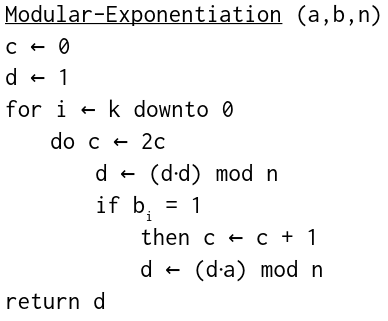
\includegraphics[scale=0.8]{esercizio17/images/mod_exp.png}
	\caption{Algoritmo per modular exponentiational di un messaggio}
	\label{fig:Mod_exp}
\end{figure}

L ' algoritmo cicla sul numero di bit dell ' esponente, moltiplica
il valore d prima per se stesso e ne fa il modulo, questo stesso valore
di d per la base quando il valore dell' esponente in forma binaria
assume valore uno e ne effettua il modulo, (il parametro c non occorre
per il calcolo del valore finale, occorre solo a capire in realt�
alla fine se il numero � stato elevato per il corretto esponente). 

\begin{figure}[H]
	\centering
	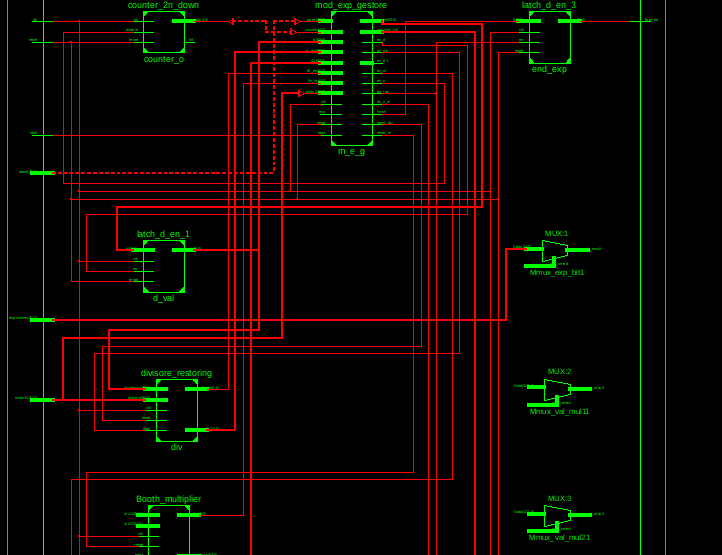
\includegraphics[scale=0.6]{esercizio17/images/exp.png}
	\caption{Hardware Exponentiational}
\end{figure}

Utiliziamo questo algoritmo perch� ci permette di riutilizzare componenti
gi� sviluppati negli esercizi precedenti, difatti osservando lo schematico,
vi � presente un moltiplicatore di Booth e il divisore restoring per
le varie operazioni prodotto e modulo, un contatore down per indicare
quale dei bit dell' esponente dobbiamo analizzare e dei selettori
descritti con il costrutto with select per selezionare quali valori
devono essere moltiplicati. La macchina a stati finiti non fa altro
che eseguire i vari passi dell' algoritmo, per� per problemi relativi
al timing � stata realizzata alla fine con un singolo process, difatti
una prima realizzazione con due process determinava che alcuni registri
contenti i dati dell' operazione assumessero un valore indefinito
(veniva sintetizzata un macchina che doveva avere una frequenza di
clock minore da quella generabile dalla scheda). 

Per problemi di spazio, si � ricorsi a componenti per la moltiplicazione
e divisione seriali, oltre ad riutilizzarli all' interno dello stesso
progetto difatti il moltiplicatore di Booth � stato utilizzato per:
calcolare il prodotto di pq ed l' esponenziazione.

\subsection{Codice}

\href{run:progetti/RSA/RSA.xise}{RSA ISE}

\selectlanguage{italian}%



\selectlanguage{italian}%

\section{Simulazione}

\begin{figure}[H]
	\centering
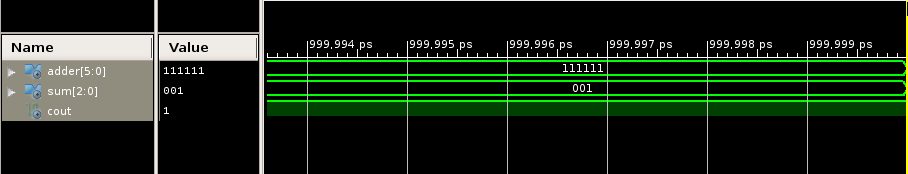
\includegraphics[scale=0.55]{esercizio10/images/carry_save_adder_testbench.png}
	\caption{Carry Save Adder}
\end{figure}\selectlanguage{italian}%



\selectlanguage{italian}%

\section{Sintesi su board FPGA}

Valgono le stesse considerazioni fatte per il Ripple Carry Adder \ref{Sintesi ripple carry},
con la differenza che ci sono sette registri da poter caricare.\selectlanguage{italian}%

\selectlanguage{italian}%



\chapter{Addizionatore a 7 operandi}

\selectlanguage{american}%

\AddToShipoutPicture{\BackgroundPicture{logo.png}{0}}

\selectlanguage{italian}%

\section{Traccia}

Realizzare un dispositivo VHDL che implementa il protocollo UART (a
partire da quello diffuso dalla Digilent). Collegare internamente,
oppure tramite inter- faccia fisica esterna alla board stessa, ad
un\textquoteright altra board oppure ad un PC previo utilizzo di un
physical RS232, due interfacce per trasmette e ricevere ottetti. Svolgere
l\textquoteright esercizio riutilizzando il VHDL messo a disposizione
da Digilent (e disponbile nel materiale del corso) commentando eventuali
ristrutturazioni del codice. (Opzionale) Sviluppare un\textquoteright architettura
per l\textquoteright implementazione del protocollo UART secondo il
paradigma PO/PC ex-novo, evidenziando le similarit`a/dissimilarit`a
con il progetto Digilent.\selectlanguage{italian}%



\selectlanguage{italian}%

\section{Soluzione}


\subsection{Schematici}

Il seguente circuito implementa l' algortimo RSA per la firma di un
messaggio, applica una funzione di hash sul messaggio e verifica che
il messaggio ricevuto sia coretto.

L' intera procedura � divisa nelle seguenti fasi: 
\begin{itemize}
\item vengono scelti i valori caratteristici per inviare il dato (p pari
a 3, q 11, e 7 e d 3) ed il messaggio da inviare;
\item si applica la funzione di hashing sul messaggio, utilizzando il metodo
della moltiplicazione;
\item viene applicata la firma sul messaggio originale utilizzando la chiave
privata, il trasmettitore invia i due dati appena calcolati (anche
se non � presente un vero e proprio invio essendo trasmettitore e
ricevitore implementati sulla stessa board);
\item Il ricevitore applica la chiave pubblica sul messaggio firmato, ne
effettua l' hashing e verifica se la sua versione del messaggio a
cui � stato applicato l' hashing � identico a quello che � stato ricevuto.
\end{itemize}
Cos� facendo garantiamo sia la segretezza( infatti non mandiamo il
messaggio in chiaro), sia l' autenticazione( chi riceve il messaggio
pu� verificare effettuando l' hashing con parametri convenuti non
� stato modificato),

Di seguito vengono descritte le varie componenti che vengono utilizzate
per effettuare l' hashing e firmare il messaggio.

\subsubsection{Funzione hash}

\begin{figure}[H]
	\centering
	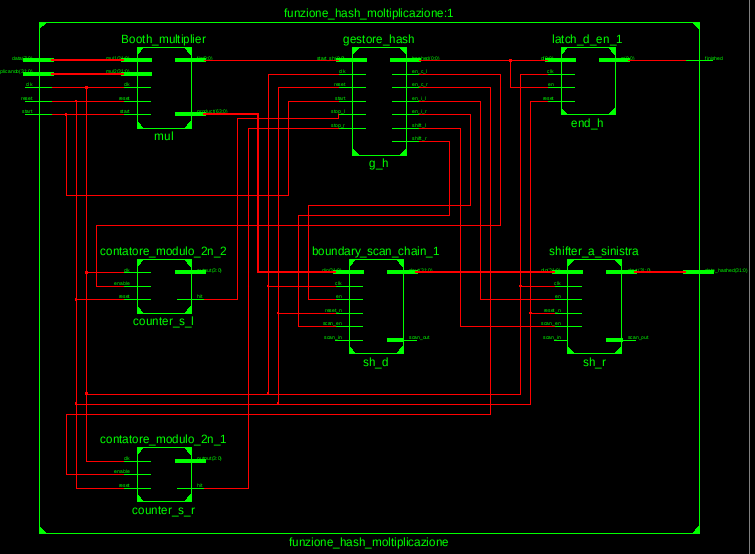
\includegraphics[scale=0.6]{esercizio17/images/hash.png}
	\caption{hasher}
	\label{fig:Mod_exp}
\end{figure}Il circuito � stato realizzato in due differenti modi: 
\begin{itemize}
\item nel primo caso si utilizza una macchina a stati finiti descritta da
cinque stati: 
\begin{itemize}
\item idle, stato di riposo dell' automa; 
\item init in cui si attende che il moltiplicatore termini il suo compito; 
\item shifting\_r in cui il valore della moltiplicazione viene shiftato
a destra; 
\item shifting\_l il valore viene shiftato a sinistra; ended per comunicare
la fine dell' operazione di hash;
\end{itemize}
\item nel secondo si � utilizzato lo stesso procedimento ma il tutto viene
implementato in un process.
\end{itemize}
Viene utilizzata la seconda soluzione perch� occupa meno spazio, dato
che le operazioni di shifting consistono semplicemente, nel caso dello
shifting a destra prendere i sedici bit pi� significativi dal risultato
della moltiplicazione, quando si shifta a sinistra basta accodare
sedici zeri per avere lo stesso risultato della prima soluzione.

Il circito viene cos� descritto poich� tale forma di hashing prevedere
di moltiplicare il dato per un valore A il quale � un numero compreso
tra 0 ed 1, di cui il denominatore � un multiplo di due, per tale
ragione di � scelto di moltiplicare per un valore W ed infine di shiftare
a destra un numero di volte pari al valore dell' esponente, tale numero
� la parte decimale del valore del dato per W (perch� quando shiftiamo
inseriamo degli zero fittizzi), dopodich� si effettua uno shifting
a sinistra di un numero pari di volte affinch� la nostra parte deciamale
rientri nella parte del registro da inviare.

\subsubsection{Esponenziatore}

Per effettuare l' elevazione a potenza con il modulo, ci siamo riferiti
a questo algoritmo :

\begin{figure}[H]
	\centering
	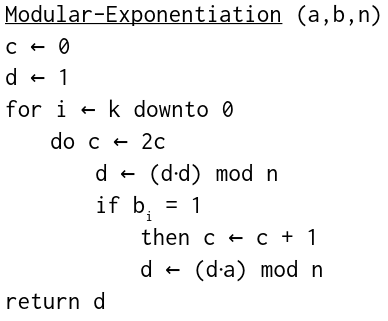
\includegraphics[scale=0.8]{esercizio17/images/mod_exp.png}
	\caption{Algoritmo per modular exponentiational di un messaggio}
	\label{fig:Mod_exp}
\end{figure}

L ' algoritmo cicla sul numero di bit dell ' esponente, moltiplica
il valore d prima per se stesso e ne fa il modulo, questo stesso valore
di d per la base quando il valore dell' esponente in forma binaria
assume valore uno e ne effettua il modulo, (il parametro c non occorre
per il calcolo del valore finale, occorre solo a capire in realt�
alla fine se il numero � stato elevato per il corretto esponente). 

\begin{figure}[H]
	\centering
	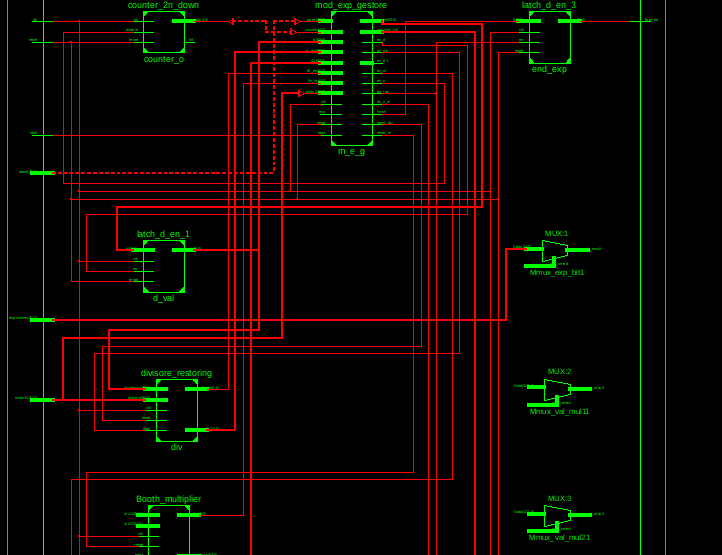
\includegraphics[scale=0.6]{esercizio17/images/exp.png}
	\caption{Hardware Exponentiational}
\end{figure}

Utiliziamo questo algoritmo perch� ci permette di riutilizzare componenti
gi� sviluppati negli esercizi precedenti, difatti osservando lo schematico,
vi � presente un moltiplicatore di Booth e il divisore restoring per
le varie operazioni prodotto e modulo, un contatore down per indicare
quale dei bit dell' esponente dobbiamo analizzare e dei selettori
descritti con il costrutto with select per selezionare quali valori
devono essere moltiplicati. La macchina a stati finiti non fa altro
che eseguire i vari passi dell' algoritmo, per� per problemi relativi
al timing � stata realizzata alla fine con un singolo process, difatti
una prima realizzazione con due process determinava che alcuni registri
contenti i dati dell' operazione assumessero un valore indefinito
(veniva sintetizzata un macchina che doveva avere una frequenza di
clock minore da quella generabile dalla scheda). 

Per problemi di spazio, si � ricorsi a componenti per la moltiplicazione
e divisione seriali, oltre ad riutilizzarli all' interno dello stesso
progetto difatti il moltiplicatore di Booth � stato utilizzato per:
calcolare il prodotto di pq ed l' esponenziazione.

\subsection{Codice}

\href{run:progetti/RSA/RSA.xise}{RSA ISE}

\selectlanguage{italian}%



\selectlanguage{italian}%

\section{Simulazione}

\begin{figure}[H]
	\centering
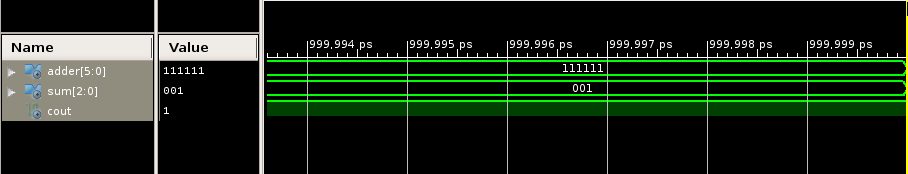
\includegraphics[scale=0.55]{esercizio10/images/carry_save_adder_testbench.png}
	\caption{Carry Save Adder}
\end{figure}\selectlanguage{italian}%



\selectlanguage{italian}%

\section{Sintesi su board FPGA}

Valgono le stesse considerazioni fatte per il Ripple Carry Adder \ref{Sintesi ripple carry},
con la differenza che ci sono sette registri da poter caricare.\selectlanguage{italian}%

\selectlanguage{italian}%



\chapter{Moltiplicatori}

\selectlanguage{american}%

\AddToShipoutPicture{\BackgroundPicture{logo.png}{0}}

\selectlanguage{italian}%

\section{Traccia}

Realizzare un dispositivo VHDL che implementa il protocollo UART (a
partire da quello diffuso dalla Digilent). Collegare internamente,
oppure tramite inter- faccia fisica esterna alla board stessa, ad
un\textquoteright altra board oppure ad un PC previo utilizzo di un
physical RS232, due interfacce per trasmette e ricevere ottetti. Svolgere
l\textquoteright esercizio riutilizzando il VHDL messo a disposizione
da Digilent (e disponbile nel materiale del corso) commentando eventuali
ristrutturazioni del codice. (Opzionale) Sviluppare un\textquoteright architettura
per l\textquoteright implementazione del protocollo UART secondo il
paradigma PO/PC ex-novo, evidenziando le similarit`a/dissimilarit`a
con il progetto Digilent.\selectlanguage{italian}%



\selectlanguage{italian}%

\section{Soluzione}


\subsection{Schematici}

Il seguente circuito implementa l' algortimo RSA per la firma di un
messaggio, applica una funzione di hash sul messaggio e verifica che
il messaggio ricevuto sia coretto.

L' intera procedura � divisa nelle seguenti fasi: 
\begin{itemize}
\item vengono scelti i valori caratteristici per inviare il dato (p pari
a 3, q 11, e 7 e d 3) ed il messaggio da inviare;
\item si applica la funzione di hashing sul messaggio, utilizzando il metodo
della moltiplicazione;
\item viene applicata la firma sul messaggio originale utilizzando la chiave
privata, il trasmettitore invia i due dati appena calcolati (anche
se non � presente un vero e proprio invio essendo trasmettitore e
ricevitore implementati sulla stessa board);
\item Il ricevitore applica la chiave pubblica sul messaggio firmato, ne
effettua l' hashing e verifica se la sua versione del messaggio a
cui � stato applicato l' hashing � identico a quello che � stato ricevuto.
\end{itemize}
Cos� facendo garantiamo sia la segretezza( infatti non mandiamo il
messaggio in chiaro), sia l' autenticazione( chi riceve il messaggio
pu� verificare effettuando l' hashing con parametri convenuti non
� stato modificato),

Di seguito vengono descritte le varie componenti che vengono utilizzate
per effettuare l' hashing e firmare il messaggio.

\subsubsection{Funzione hash}

\begin{figure}[H]
	\centering
	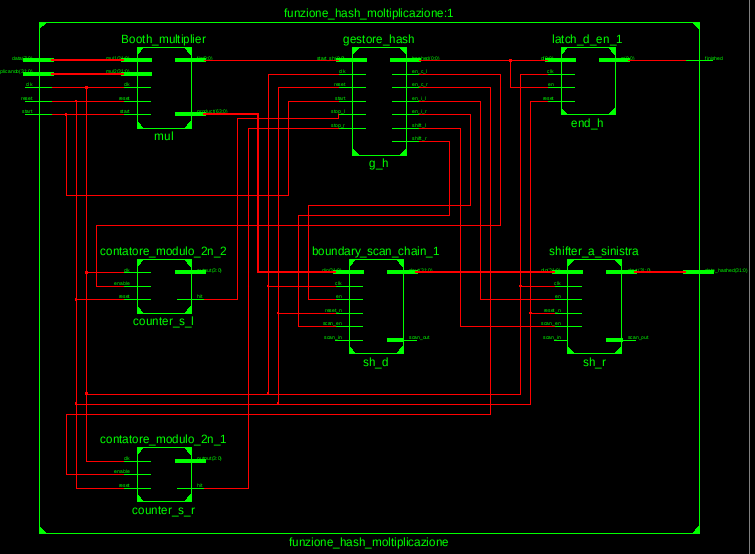
\includegraphics[scale=0.6]{esercizio17/images/hash.png}
	\caption{hasher}
	\label{fig:Mod_exp}
\end{figure}Il circuito � stato realizzato in due differenti modi: 
\begin{itemize}
\item nel primo caso si utilizza una macchina a stati finiti descritta da
cinque stati: 
\begin{itemize}
\item idle, stato di riposo dell' automa; 
\item init in cui si attende che il moltiplicatore termini il suo compito; 
\item shifting\_r in cui il valore della moltiplicazione viene shiftato
a destra; 
\item shifting\_l il valore viene shiftato a sinistra; ended per comunicare
la fine dell' operazione di hash;
\end{itemize}
\item nel secondo si � utilizzato lo stesso procedimento ma il tutto viene
implementato in un process.
\end{itemize}
Viene utilizzata la seconda soluzione perch� occupa meno spazio, dato
che le operazioni di shifting consistono semplicemente, nel caso dello
shifting a destra prendere i sedici bit pi� significativi dal risultato
della moltiplicazione, quando si shifta a sinistra basta accodare
sedici zeri per avere lo stesso risultato della prima soluzione.

Il circito viene cos� descritto poich� tale forma di hashing prevedere
di moltiplicare il dato per un valore A il quale � un numero compreso
tra 0 ed 1, di cui il denominatore � un multiplo di due, per tale
ragione di � scelto di moltiplicare per un valore W ed infine di shiftare
a destra un numero di volte pari al valore dell' esponente, tale numero
� la parte decimale del valore del dato per W (perch� quando shiftiamo
inseriamo degli zero fittizzi), dopodich� si effettua uno shifting
a sinistra di un numero pari di volte affinch� la nostra parte deciamale
rientri nella parte del registro da inviare.

\subsubsection{Esponenziatore}

Per effettuare l' elevazione a potenza con il modulo, ci siamo riferiti
a questo algoritmo :

\begin{figure}[H]
	\centering
	\includegraphics[scale=0.8]{esercizio17/images/mod_exp.png}
	\caption{Algoritmo per modular exponentiational di un messaggio}
	\label{fig:Mod_exp}
\end{figure}

L ' algoritmo cicla sul numero di bit dell ' esponente, moltiplica
il valore d prima per se stesso e ne fa il modulo, questo stesso valore
di d per la base quando il valore dell' esponente in forma binaria
assume valore uno e ne effettua il modulo, (il parametro c non occorre
per il calcolo del valore finale, occorre solo a capire in realt�
alla fine se il numero � stato elevato per il corretto esponente). 

\begin{figure}[H]
	\centering
	\includegraphics[scale=0.6]{esercizio17/images/exp.png}
	\caption{Hardware Exponentiational}
\end{figure}

Utiliziamo questo algoritmo perch� ci permette di riutilizzare componenti
gi� sviluppati negli esercizi precedenti, difatti osservando lo schematico,
vi � presente un moltiplicatore di Booth e il divisore restoring per
le varie operazioni prodotto e modulo, un contatore down per indicare
quale dei bit dell' esponente dobbiamo analizzare e dei selettori
descritti con il costrutto with select per selezionare quali valori
devono essere moltiplicati. La macchina a stati finiti non fa altro
che eseguire i vari passi dell' algoritmo, per� per problemi relativi
al timing � stata realizzata alla fine con un singolo process, difatti
una prima realizzazione con due process determinava che alcuni registri
contenti i dati dell' operazione assumessero un valore indefinito
(veniva sintetizzata un macchina che doveva avere una frequenza di
clock minore da quella generabile dalla scheda). 

Per problemi di spazio, si � ricorsi a componenti per la moltiplicazione
e divisione seriali, oltre ad riutilizzarli all' interno dello stesso
progetto difatti il moltiplicatore di Booth � stato utilizzato per:
calcolare il prodotto di pq ed l' esponenziazione.

\subsection{Codice}

\href{run:progetti/RSA/RSA.xise}{RSA ISE}

\selectlanguage{italian}%



\selectlanguage{italian}%

\section{Simulazione}

\begin{figure}[H]
	\centering
\includegraphics[scale=0.55]{esercizio10/images/carry_save_adder_testbench.png}
	\caption{Carry Save Adder}
\end{figure}\selectlanguage{italian}%



\selectlanguage{italian}%

\section{Sintesi su board FPGA}

Valgono le stesse considerazioni fatte per il Ripple Carry Adder \ref{Sintesi ripple carry},
con la differenza che ci sono sette registri da poter caricare.\selectlanguage{italian}%

\selectlanguage{italian}%



\chapter{Divisori}

\selectlanguage{american}%

\AddToShipoutPicture{\BackgroundPicture{logo.png}{0}}

\selectlanguage{italian}%

\section{Traccia}

Realizzare un dispositivo VHDL che implementa il protocollo UART (a
partire da quello diffuso dalla Digilent). Collegare internamente,
oppure tramite inter- faccia fisica esterna alla board stessa, ad
un\textquoteright altra board oppure ad un PC previo utilizzo di un
physical RS232, due interfacce per trasmette e ricevere ottetti. Svolgere
l\textquoteright esercizio riutilizzando il VHDL messo a disposizione
da Digilent (e disponbile nel materiale del corso) commentando eventuali
ristrutturazioni del codice. (Opzionale) Sviluppare un\textquoteright architettura
per l\textquoteright implementazione del protocollo UART secondo il
paradigma PO/PC ex-novo, evidenziando le similarit`a/dissimilarit`a
con il progetto Digilent.\selectlanguage{italian}%



\selectlanguage{italian}%

\section{Soluzione}


\subsection{Schematici}

Il seguente circuito implementa l' algortimo RSA per la firma di un
messaggio, applica una funzione di hash sul messaggio e verifica che
il messaggio ricevuto sia coretto.

L' intera procedura � divisa nelle seguenti fasi: 
\begin{itemize}
\item vengono scelti i valori caratteristici per inviare il dato (p pari
a 3, q 11, e 7 e d 3) ed il messaggio da inviare;
\item si applica la funzione di hashing sul messaggio, utilizzando il metodo
della moltiplicazione;
\item viene applicata la firma sul messaggio originale utilizzando la chiave
privata, il trasmettitore invia i due dati appena calcolati (anche
se non � presente un vero e proprio invio essendo trasmettitore e
ricevitore implementati sulla stessa board);
\item Il ricevitore applica la chiave pubblica sul messaggio firmato, ne
effettua l' hashing e verifica se la sua versione del messaggio a
cui � stato applicato l' hashing � identico a quello che � stato ricevuto.
\end{itemize}
Cos� facendo garantiamo sia la segretezza( infatti non mandiamo il
messaggio in chiaro), sia l' autenticazione( chi riceve il messaggio
pu� verificare effettuando l' hashing con parametri convenuti non
� stato modificato),

Di seguito vengono descritte le varie componenti che vengono utilizzate
per effettuare l' hashing e firmare il messaggio.

\subsubsection{Funzione hash}

\begin{figure}[H]
	\centering
	\includegraphics[scale=0.6]{esercizio17/images/hash.png}
	\caption{hasher}
	\label{fig:Mod_exp}
\end{figure}Il circuito � stato realizzato in due differenti modi: 
\begin{itemize}
\item nel primo caso si utilizza una macchina a stati finiti descritta da
cinque stati: 
\begin{itemize}
\item idle, stato di riposo dell' automa; 
\item init in cui si attende che il moltiplicatore termini il suo compito; 
\item shifting\_r in cui il valore della moltiplicazione viene shiftato
a destra; 
\item shifting\_l il valore viene shiftato a sinistra; ended per comunicare
la fine dell' operazione di hash;
\end{itemize}
\item nel secondo si � utilizzato lo stesso procedimento ma il tutto viene
implementato in un process.
\end{itemize}
Viene utilizzata la seconda soluzione perch� occupa meno spazio, dato
che le operazioni di shifting consistono semplicemente, nel caso dello
shifting a destra prendere i sedici bit pi� significativi dal risultato
della moltiplicazione, quando si shifta a sinistra basta accodare
sedici zeri per avere lo stesso risultato della prima soluzione.

Il circito viene cos� descritto poich� tale forma di hashing prevedere
di moltiplicare il dato per un valore A il quale � un numero compreso
tra 0 ed 1, di cui il denominatore � un multiplo di due, per tale
ragione di � scelto di moltiplicare per un valore W ed infine di shiftare
a destra un numero di volte pari al valore dell' esponente, tale numero
� la parte decimale del valore del dato per W (perch� quando shiftiamo
inseriamo degli zero fittizzi), dopodich� si effettua uno shifting
a sinistra di un numero pari di volte affinch� la nostra parte deciamale
rientri nella parte del registro da inviare.

\subsubsection{Esponenziatore}

Per effettuare l' elevazione a potenza con il modulo, ci siamo riferiti
a questo algoritmo :

\begin{figure}[H]
	\centering
	\includegraphics[scale=0.8]{esercizio17/images/mod_exp.png}
	\caption{Algoritmo per modular exponentiational di un messaggio}
	\label{fig:Mod_exp}
\end{figure}

L ' algoritmo cicla sul numero di bit dell ' esponente, moltiplica
il valore d prima per se stesso e ne fa il modulo, questo stesso valore
di d per la base quando il valore dell' esponente in forma binaria
assume valore uno e ne effettua il modulo, (il parametro c non occorre
per il calcolo del valore finale, occorre solo a capire in realt�
alla fine se il numero � stato elevato per il corretto esponente). 

\begin{figure}[H]
	\centering
	\includegraphics[scale=0.6]{esercizio17/images/exp.png}
	\caption{Hardware Exponentiational}
\end{figure}

Utiliziamo questo algoritmo perch� ci permette di riutilizzare componenti
gi� sviluppati negli esercizi precedenti, difatti osservando lo schematico,
vi � presente un moltiplicatore di Booth e il divisore restoring per
le varie operazioni prodotto e modulo, un contatore down per indicare
quale dei bit dell' esponente dobbiamo analizzare e dei selettori
descritti con il costrutto with select per selezionare quali valori
devono essere moltiplicati. La macchina a stati finiti non fa altro
che eseguire i vari passi dell' algoritmo, per� per problemi relativi
al timing � stata realizzata alla fine con un singolo process, difatti
una prima realizzazione con due process determinava che alcuni registri
contenti i dati dell' operazione assumessero un valore indefinito
(veniva sintetizzata un macchina che doveva avere una frequenza di
clock minore da quella generabile dalla scheda). 

Per problemi di spazio, si � ricorsi a componenti per la moltiplicazione
e divisione seriali, oltre ad riutilizzarli all' interno dello stesso
progetto difatti il moltiplicatore di Booth � stato utilizzato per:
calcolare il prodotto di pq ed l' esponenziazione.

\subsection{Codice}

\href{run:progetti/RSA/RSA.xise}{RSA ISE}

\selectlanguage{italian}%



\selectlanguage{italian}%

\section{Simulazione}

\begin{figure}[H]
	\centering
\includegraphics[scale=0.55]{esercizio10/images/carry_save_adder_testbench.png}
	\caption{Carry Save Adder}
\end{figure}\selectlanguage{italian}%



\selectlanguage{italian}%

\section{Sintesi su board FPGA}

Valgono le stesse considerazioni fatte per il Ripple Carry Adder \ref{Sintesi ripple carry},
con la differenza che ci sono sette registri da poter caricare.\selectlanguage{italian}%

\selectlanguage{italian}%



\chapter{UART}

\selectlanguage{american}%

\AddToShipoutPicture{\BackgroundPicture{logo.png}{0}}

\selectlanguage{italian}%

\section{Traccia}

Realizzare un dispositivo VHDL che implementa il protocollo UART (a
partire da quello diffuso dalla Digilent). Collegare internamente,
oppure tramite inter- faccia fisica esterna alla board stessa, ad
un\textquoteright altra board oppure ad un PC previo utilizzo di un
physical RS232, due interfacce per trasmette e ricevere ottetti. Svolgere
l\textquoteright esercizio riutilizzando il VHDL messo a disposizione
da Digilent (e disponbile nel materiale del corso) commentando eventuali
ristrutturazioni del codice. (Opzionale) Sviluppare un\textquoteright architettura
per l\textquoteright implementazione del protocollo UART secondo il
paradigma PO/PC ex-novo, evidenziando le similarit`a/dissimilarit`a
con il progetto Digilent.\selectlanguage{italian}%



\selectlanguage{italian}%

\section{Soluzione}


\subsection{Schematici}

Il seguente circuito implementa l' algortimo RSA per la firma di un
messaggio, applica una funzione di hash sul messaggio e verifica che
il messaggio ricevuto sia coretto.

L' intera procedura � divisa nelle seguenti fasi: 
\begin{itemize}
\item vengono scelti i valori caratteristici per inviare il dato (p pari
a 3, q 11, e 7 e d 3) ed il messaggio da inviare;
\item si applica la funzione di hashing sul messaggio, utilizzando il metodo
della moltiplicazione;
\item viene applicata la firma sul messaggio originale utilizzando la chiave
privata, il trasmettitore invia i due dati appena calcolati (anche
se non � presente un vero e proprio invio essendo trasmettitore e
ricevitore implementati sulla stessa board);
\item Il ricevitore applica la chiave pubblica sul messaggio firmato, ne
effettua l' hashing e verifica se la sua versione del messaggio a
cui � stato applicato l' hashing � identico a quello che � stato ricevuto.
\end{itemize}
Cos� facendo garantiamo sia la segretezza( infatti non mandiamo il
messaggio in chiaro), sia l' autenticazione( chi riceve il messaggio
pu� verificare effettuando l' hashing con parametri convenuti non
� stato modificato),

Di seguito vengono descritte le varie componenti che vengono utilizzate
per effettuare l' hashing e firmare il messaggio.

\subsubsection{Funzione hash}

\begin{figure}[H]
	\centering
	\includegraphics[scale=0.6]{esercizio17/images/hash.png}
	\caption{hasher}
	\label{fig:Mod_exp}
\end{figure}Il circuito � stato realizzato in due differenti modi: 
\begin{itemize}
\item nel primo caso si utilizza una macchina a stati finiti descritta da
cinque stati: 
\begin{itemize}
\item idle, stato di riposo dell' automa; 
\item init in cui si attende che il moltiplicatore termini il suo compito; 
\item shifting\_r in cui il valore della moltiplicazione viene shiftato
a destra; 
\item shifting\_l il valore viene shiftato a sinistra; ended per comunicare
la fine dell' operazione di hash;
\end{itemize}
\item nel secondo si � utilizzato lo stesso procedimento ma il tutto viene
implementato in un process.
\end{itemize}
Viene utilizzata la seconda soluzione perch� occupa meno spazio, dato
che le operazioni di shifting consistono semplicemente, nel caso dello
shifting a destra prendere i sedici bit pi� significativi dal risultato
della moltiplicazione, quando si shifta a sinistra basta accodare
sedici zeri per avere lo stesso risultato della prima soluzione.

Il circito viene cos� descritto poich� tale forma di hashing prevedere
di moltiplicare il dato per un valore A il quale � un numero compreso
tra 0 ed 1, di cui il denominatore � un multiplo di due, per tale
ragione di � scelto di moltiplicare per un valore W ed infine di shiftare
a destra un numero di volte pari al valore dell' esponente, tale numero
� la parte decimale del valore del dato per W (perch� quando shiftiamo
inseriamo degli zero fittizzi), dopodich� si effettua uno shifting
a sinistra di un numero pari di volte affinch� la nostra parte deciamale
rientri nella parte del registro da inviare.

\subsubsection{Esponenziatore}

Per effettuare l' elevazione a potenza con il modulo, ci siamo riferiti
a questo algoritmo :

\begin{figure}[H]
	\centering
	\includegraphics[scale=0.8]{esercizio17/images/mod_exp.png}
	\caption{Algoritmo per modular exponentiational di un messaggio}
	\label{fig:Mod_exp}
\end{figure}

L ' algoritmo cicla sul numero di bit dell ' esponente, moltiplica
il valore d prima per se stesso e ne fa il modulo, questo stesso valore
di d per la base quando il valore dell' esponente in forma binaria
assume valore uno e ne effettua il modulo, (il parametro c non occorre
per il calcolo del valore finale, occorre solo a capire in realt�
alla fine se il numero � stato elevato per il corretto esponente). 

\begin{figure}[H]
	\centering
	\includegraphics[scale=0.6]{esercizio17/images/exp.png}
	\caption{Hardware Exponentiational}
\end{figure}

Utiliziamo questo algoritmo perch� ci permette di riutilizzare componenti
gi� sviluppati negli esercizi precedenti, difatti osservando lo schematico,
vi � presente un moltiplicatore di Booth e il divisore restoring per
le varie operazioni prodotto e modulo, un contatore down per indicare
quale dei bit dell' esponente dobbiamo analizzare e dei selettori
descritti con il costrutto with select per selezionare quali valori
devono essere moltiplicati. La macchina a stati finiti non fa altro
che eseguire i vari passi dell' algoritmo, per� per problemi relativi
al timing � stata realizzata alla fine con un singolo process, difatti
una prima realizzazione con due process determinava che alcuni registri
contenti i dati dell' operazione assumessero un valore indefinito
(veniva sintetizzata un macchina che doveva avere una frequenza di
clock minore da quella generabile dalla scheda). 

Per problemi di spazio, si � ricorsi a componenti per la moltiplicazione
e divisione seriali, oltre ad riutilizzarli all' interno dello stesso
progetto difatti il moltiplicatore di Booth � stato utilizzato per:
calcolare il prodotto di pq ed l' esponenziazione.

\subsection{Codice}

\href{run:progetti/RSA/RSA.xise}{RSA ISE}

\selectlanguage{italian}%



\selectlanguage{italian}%

\section{Simulazione}

\begin{figure}[H]
	\centering
\includegraphics[scale=0.55]{esercizio10/images/carry_save_adder_testbench.png}
	\caption{Carry Save Adder}
\end{figure}\selectlanguage{italian}%



\selectlanguage{italian}%

\section{Sintesi su board FPGA}

Valgono le stesse considerazioni fatte per il Ripple Carry Adder \ref{Sintesi ripple carry},
con la differenza che ci sono sette registri da poter caricare.\selectlanguage{italian}%

\selectlanguage{italian}%



\chapter{GPIO}

\selectlanguage{american}%

\AddToShipoutPicture{\BackgroundPicture{logo.png}{0}}

\selectlanguage{italian}%

\section{Traccia}

Realizzare un dispositivo VHDL che implementa il protocollo UART (a
partire da quello diffuso dalla Digilent). Collegare internamente,
oppure tramite inter- faccia fisica esterna alla board stessa, ad
un\textquoteright altra board oppure ad un PC previo utilizzo di un
physical RS232, due interfacce per trasmette e ricevere ottetti. Svolgere
l\textquoteright esercizio riutilizzando il VHDL messo a disposizione
da Digilent (e disponbile nel materiale del corso) commentando eventuali
ristrutturazioni del codice. (Opzionale) Sviluppare un\textquoteright architettura
per l\textquoteright implementazione del protocollo UART secondo il
paradigma PO/PC ex-novo, evidenziando le similarit`a/dissimilarit`a
con il progetto Digilent.\selectlanguage{italian}%



\selectlanguage{italian}%

\section{Soluzione}


\subsection{Schematici}

Il seguente circuito implementa l' algortimo RSA per la firma di un
messaggio, applica una funzione di hash sul messaggio e verifica che
il messaggio ricevuto sia coretto.

L' intera procedura � divisa nelle seguenti fasi: 
\begin{itemize}
\item vengono scelti i valori caratteristici per inviare il dato (p pari
a 3, q 11, e 7 e d 3) ed il messaggio da inviare;
\item si applica la funzione di hashing sul messaggio, utilizzando il metodo
della moltiplicazione;
\item viene applicata la firma sul messaggio originale utilizzando la chiave
privata, il trasmettitore invia i due dati appena calcolati (anche
se non � presente un vero e proprio invio essendo trasmettitore e
ricevitore implementati sulla stessa board);
\item Il ricevitore applica la chiave pubblica sul messaggio firmato, ne
effettua l' hashing e verifica se la sua versione del messaggio a
cui � stato applicato l' hashing � identico a quello che � stato ricevuto.
\end{itemize}
Cos� facendo garantiamo sia la segretezza( infatti non mandiamo il
messaggio in chiaro), sia l' autenticazione( chi riceve il messaggio
pu� verificare effettuando l' hashing con parametri convenuti non
� stato modificato),

Di seguito vengono descritte le varie componenti che vengono utilizzate
per effettuare l' hashing e firmare il messaggio.

\subsubsection{Funzione hash}

\begin{figure}[H]
	\centering
	\includegraphics[scale=0.6]{esercizio17/images/hash.png}
	\caption{hasher}
	\label{fig:Mod_exp}
\end{figure}Il circuito � stato realizzato in due differenti modi: 
\begin{itemize}
\item nel primo caso si utilizza una macchina a stati finiti descritta da
cinque stati: 
\begin{itemize}
\item idle, stato di riposo dell' automa; 
\item init in cui si attende che il moltiplicatore termini il suo compito; 
\item shifting\_r in cui il valore della moltiplicazione viene shiftato
a destra; 
\item shifting\_l il valore viene shiftato a sinistra; ended per comunicare
la fine dell' operazione di hash;
\end{itemize}
\item nel secondo si � utilizzato lo stesso procedimento ma il tutto viene
implementato in un process.
\end{itemize}
Viene utilizzata la seconda soluzione perch� occupa meno spazio, dato
che le operazioni di shifting consistono semplicemente, nel caso dello
shifting a destra prendere i sedici bit pi� significativi dal risultato
della moltiplicazione, quando si shifta a sinistra basta accodare
sedici zeri per avere lo stesso risultato della prima soluzione.

Il circito viene cos� descritto poich� tale forma di hashing prevedere
di moltiplicare il dato per un valore A il quale � un numero compreso
tra 0 ed 1, di cui il denominatore � un multiplo di due, per tale
ragione di � scelto di moltiplicare per un valore W ed infine di shiftare
a destra un numero di volte pari al valore dell' esponente, tale numero
� la parte decimale del valore del dato per W (perch� quando shiftiamo
inseriamo degli zero fittizzi), dopodich� si effettua uno shifting
a sinistra di un numero pari di volte affinch� la nostra parte deciamale
rientri nella parte del registro da inviare.

\subsubsection{Esponenziatore}

Per effettuare l' elevazione a potenza con il modulo, ci siamo riferiti
a questo algoritmo :

\begin{figure}[H]
	\centering
	\includegraphics[scale=0.8]{esercizio17/images/mod_exp.png}
	\caption{Algoritmo per modular exponentiational di un messaggio}
	\label{fig:Mod_exp}
\end{figure}

L ' algoritmo cicla sul numero di bit dell ' esponente, moltiplica
il valore d prima per se stesso e ne fa il modulo, questo stesso valore
di d per la base quando il valore dell' esponente in forma binaria
assume valore uno e ne effettua il modulo, (il parametro c non occorre
per il calcolo del valore finale, occorre solo a capire in realt�
alla fine se il numero � stato elevato per il corretto esponente). 

\begin{figure}[H]
	\centering
	\includegraphics[scale=0.6]{esercizio17/images/exp.png}
	\caption{Hardware Exponentiational}
\end{figure}

Utiliziamo questo algoritmo perch� ci permette di riutilizzare componenti
gi� sviluppati negli esercizi precedenti, difatti osservando lo schematico,
vi � presente un moltiplicatore di Booth e il divisore restoring per
le varie operazioni prodotto e modulo, un contatore down per indicare
quale dei bit dell' esponente dobbiamo analizzare e dei selettori
descritti con il costrutto with select per selezionare quali valori
devono essere moltiplicati. La macchina a stati finiti non fa altro
che eseguire i vari passi dell' algoritmo, per� per problemi relativi
al timing � stata realizzata alla fine con un singolo process, difatti
una prima realizzazione con due process determinava che alcuni registri
contenti i dati dell' operazione assumessero un valore indefinito
(veniva sintetizzata un macchina che doveva avere una frequenza di
clock minore da quella generabile dalla scheda). 

Per problemi di spazio, si � ricorsi a componenti per la moltiplicazione
e divisione seriali, oltre ad riutilizzarli all' interno dello stesso
progetto difatti il moltiplicatore di Booth � stato utilizzato per:
calcolare il prodotto di pq ed l' esponenziazione.

\subsection{Codice}

\href{run:progetti/RSA/RSA.xise}{RSA ISE}

\selectlanguage{italian}%



\selectlanguage{italian}%

\section{Simulazione}

\begin{figure}[H]
	\centering
\includegraphics[scale=0.55]{esercizio10/images/carry_save_adder_testbench.png}
	\caption{Carry Save Adder}
\end{figure}\selectlanguage{italian}%



\selectlanguage{italian}%

\section{Sintesi su board FPGA}

Valgono le stesse considerazioni fatte per il Ripple Carry Adder \ref{Sintesi ripple carry},
con la differenza che ci sono sette registri da poter caricare.\selectlanguage{italian}%

\selectlanguage{italian}%



\chapter{Firma digitale}

\selectlanguage{american}%

\AddToShipoutPicture{\BackgroundPicture{logo.png}{0}}

\selectlanguage{italian}%

\section{Traccia}

Realizzare un dispositivo VHDL che implementa il protocollo UART (a
partire da quello diffuso dalla Digilent). Collegare internamente,
oppure tramite inter- faccia fisica esterna alla board stessa, ad
un\textquoteright altra board oppure ad un PC previo utilizzo di un
physical RS232, due interfacce per trasmette e ricevere ottetti. Svolgere
l\textquoteright esercizio riutilizzando il VHDL messo a disposizione
da Digilent (e disponbile nel materiale del corso) commentando eventuali
ristrutturazioni del codice. (Opzionale) Sviluppare un\textquoteright architettura
per l\textquoteright implementazione del protocollo UART secondo il
paradigma PO/PC ex-novo, evidenziando le similarit`a/dissimilarit`a
con il progetto Digilent.\selectlanguage{italian}%



\selectlanguage{italian}%

\section{Soluzione}


\subsection{Schematici}

Il seguente circuito implementa l' algortimo RSA per la firma di un
messaggio, applica una funzione di hash sul messaggio e verifica che
il messaggio ricevuto sia coretto.

L' intera procedura � divisa nelle seguenti fasi: 
\begin{itemize}
\item vengono scelti i valori caratteristici per inviare il dato (p pari
a 3, q 11, e 7 e d 3) ed il messaggio da inviare;
\item si applica la funzione di hashing sul messaggio, utilizzando il metodo
della moltiplicazione;
\item viene applicata la firma sul messaggio originale utilizzando la chiave
privata, il trasmettitore invia i due dati appena calcolati (anche
se non � presente un vero e proprio invio essendo trasmettitore e
ricevitore implementati sulla stessa board);
\item Il ricevitore applica la chiave pubblica sul messaggio firmato, ne
effettua l' hashing e verifica se la sua versione del messaggio a
cui � stato applicato l' hashing � identico a quello che � stato ricevuto.
\end{itemize}
Cos� facendo garantiamo sia la segretezza( infatti non mandiamo il
messaggio in chiaro), sia l' autenticazione( chi riceve il messaggio
pu� verificare effettuando l' hashing con parametri convenuti non
� stato modificato),

Di seguito vengono descritte le varie componenti che vengono utilizzate
per effettuare l' hashing e firmare il messaggio.

\subsubsection{Funzione hash}

\begin{figure}[H]
	\centering
	\includegraphics[scale=0.6]{esercizio17/images/hash.png}
	\caption{hasher}
	\label{fig:Mod_exp}
\end{figure}Il circuito � stato realizzato in due differenti modi: 
\begin{itemize}
\item nel primo caso si utilizza una macchina a stati finiti descritta da
cinque stati: 
\begin{itemize}
\item idle, stato di riposo dell' automa; 
\item init in cui si attende che il moltiplicatore termini il suo compito; 
\item shifting\_r in cui il valore della moltiplicazione viene shiftato
a destra; 
\item shifting\_l il valore viene shiftato a sinistra; ended per comunicare
la fine dell' operazione di hash;
\end{itemize}
\item nel secondo si � utilizzato lo stesso procedimento ma il tutto viene
implementato in un process.
\end{itemize}
Viene utilizzata la seconda soluzione perch� occupa meno spazio, dato
che le operazioni di shifting consistono semplicemente, nel caso dello
shifting a destra prendere i sedici bit pi� significativi dal risultato
della moltiplicazione, quando si shifta a sinistra basta accodare
sedici zeri per avere lo stesso risultato della prima soluzione.

Il circito viene cos� descritto poich� tale forma di hashing prevedere
di moltiplicare il dato per un valore A il quale � un numero compreso
tra 0 ed 1, di cui il denominatore � un multiplo di due, per tale
ragione di � scelto di moltiplicare per un valore W ed infine di shiftare
a destra un numero di volte pari al valore dell' esponente, tale numero
� la parte decimale del valore del dato per W (perch� quando shiftiamo
inseriamo degli zero fittizzi), dopodich� si effettua uno shifting
a sinistra di un numero pari di volte affinch� la nostra parte deciamale
rientri nella parte del registro da inviare.

\subsubsection{Esponenziatore}

Per effettuare l' elevazione a potenza con il modulo, ci siamo riferiti
a questo algoritmo :

\begin{figure}[H]
	\centering
	\includegraphics[scale=0.8]{esercizio17/images/mod_exp.png}
	\caption{Algoritmo per modular exponentiational di un messaggio}
	\label{fig:Mod_exp}
\end{figure}

L ' algoritmo cicla sul numero di bit dell ' esponente, moltiplica
il valore d prima per se stesso e ne fa il modulo, questo stesso valore
di d per la base quando il valore dell' esponente in forma binaria
assume valore uno e ne effettua il modulo, (il parametro c non occorre
per il calcolo del valore finale, occorre solo a capire in realt�
alla fine se il numero � stato elevato per il corretto esponente). 

\begin{figure}[H]
	\centering
	\includegraphics[scale=0.6]{esercizio17/images/exp.png}
	\caption{Hardware Exponentiational}
\end{figure}

Utiliziamo questo algoritmo perch� ci permette di riutilizzare componenti
gi� sviluppati negli esercizi precedenti, difatti osservando lo schematico,
vi � presente un moltiplicatore di Booth e il divisore restoring per
le varie operazioni prodotto e modulo, un contatore down per indicare
quale dei bit dell' esponente dobbiamo analizzare e dei selettori
descritti con il costrutto with select per selezionare quali valori
devono essere moltiplicati. La macchina a stati finiti non fa altro
che eseguire i vari passi dell' algoritmo, per� per problemi relativi
al timing � stata realizzata alla fine con un singolo process, difatti
una prima realizzazione con due process determinava che alcuni registri
contenti i dati dell' operazione assumessero un valore indefinito
(veniva sintetizzata un macchina che doveva avere una frequenza di
clock minore da quella generabile dalla scheda). 

Per problemi di spazio, si � ricorsi a componenti per la moltiplicazione
e divisione seriali, oltre ad riutilizzarli all' interno dello stesso
progetto difatti il moltiplicatore di Booth � stato utilizzato per:
calcolare il prodotto di pq ed l' esponenziazione.

\subsection{Codice}

\href{run:progetti/RSA/RSA.xise}{RSA ISE}

\selectlanguage{italian}%



\selectlanguage{italian}%

\section{Simulazione}

\begin{figure}[H]
	\centering
\includegraphics[scale=0.55]{esercizio10/images/carry_save_adder_testbench.png}
	\caption{Carry Save Adder}
\end{figure}\selectlanguage{italian}%



\selectlanguage{italian}%

\section{Sintesi su board FPGA}

Valgono le stesse considerazioni fatte per il Ripple Carry Adder \ref{Sintesi ripple carry},
con la differenza che ci sono sette registri da poter caricare.\selectlanguage{italian}%

\selectlanguage{italian}%



\selectlanguage{american}%
\end{mainmatter}\selectlanguage{italian}%

\end{document}
